\chapter{Experiments and Results}
\lhead{\emph{Evaluation}}
This chapter presents the results of implementation of frontier based exploration using Wi-Coverage with a single robot, tested in different simulated environments. The simulation environments are created using Gazebo simulator. Later we discuss in detail, the technicalities faced while realizing the frontier based exploration in the real world and ways to solve them. 

\section{System Setup}
A Turtlebot configured with Kinect Xbox 360 and an Nvidia TK1 CPU is used in this work(see chapter 3). Gazebo simulation software was used for experimenting in different simulated environments. For visualizing the constructed map and for other debugging purposes such as visualizing identified frontiers, frontier selections, origin of occupancy grid, trajectory planned by move\_base, local and global costmaps, simulated AP locations, etc, Rviz has been used. The robot is equipped with SLAM packages and exploration strategies, signal strength models are varied through controller.py node in the ndrones ROS package. Results evaluated for Wi-Coverage are based on time taken to explore and percentage of area covered vs time. 

% \section{Frontier Exploration}
% \begin{figure}
%     \centering
%     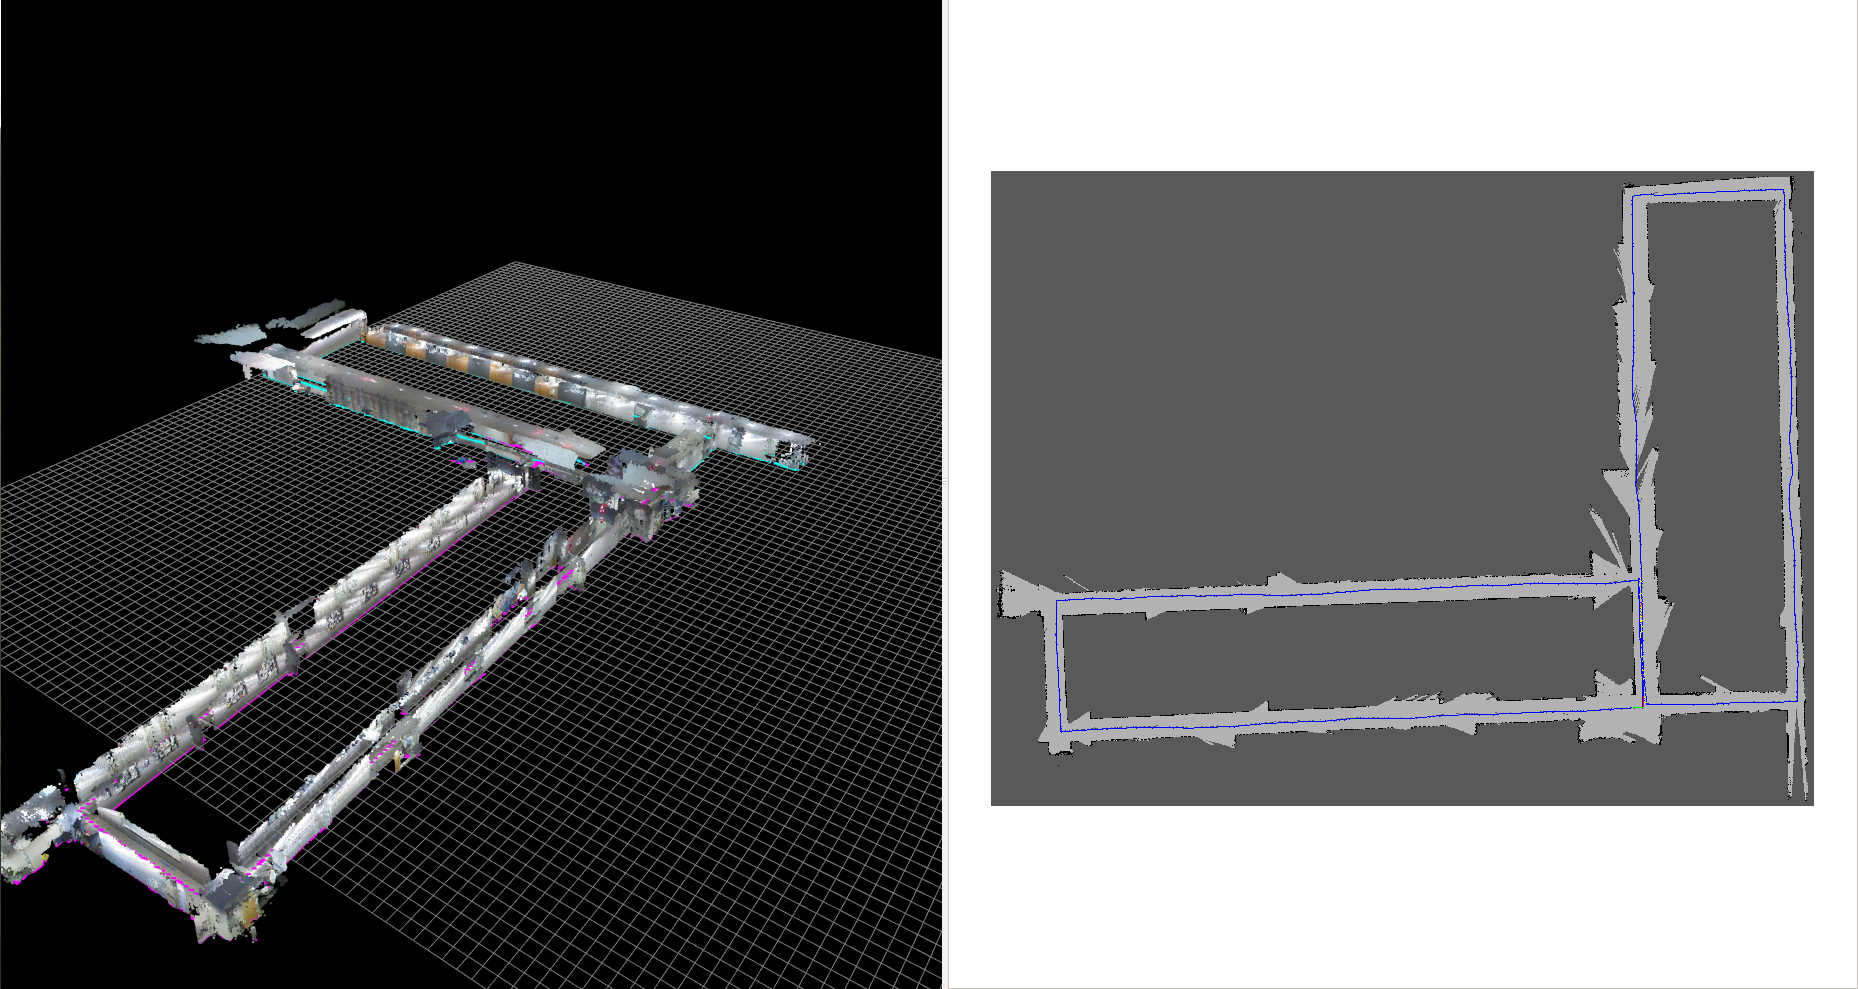
\includegraphics[width=0.75\textwidth]{images/Davis3.png}
%     \caption{Full coverage time in free space shown in Fig. xxx}
%     \label{fig:freespace}
% \end{figure}

\section{Wi-Fi}
To implement and evaluate our proposed exploration algorithm, multiple environments have been created using Gazebo simulator. Since no modules to simulate Wi-Fi APs were available we have implemented our own Wi-Fi simulation modules for the experiments. To simulate explorations in different environments using simulated Wi-Fi, we used two signal strength models, the standard ITU indoor model and a custom signal strength model from \cite{30}.

\subsection{ITU indoor Model}
\begin{figure*}[!b]
\centering
	\begin{subfigure}[b]{\textwidth}
		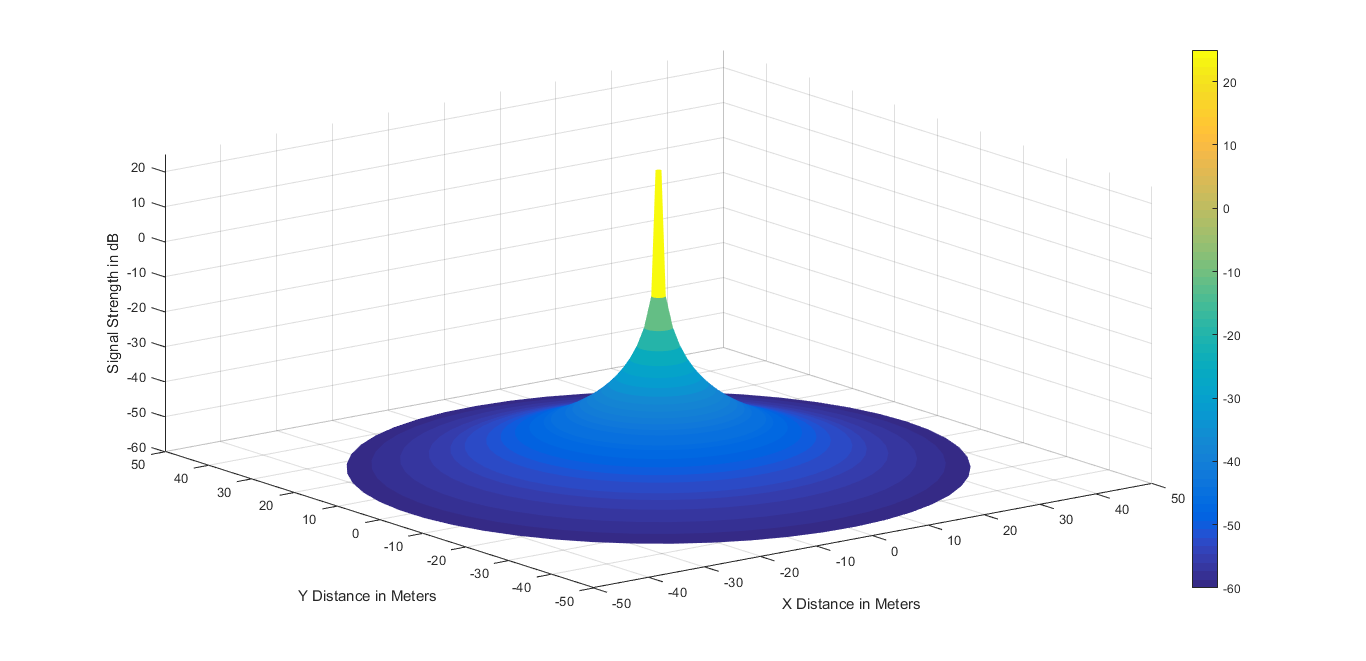
\includegraphics[width=\textwidth]{images/ITU_rm_3d.png}
		\label{subfig:a}
		\caption{}
	\end{subfigure}
    % \vfill
	\begin{subfigure}[b]{\textwidth}
		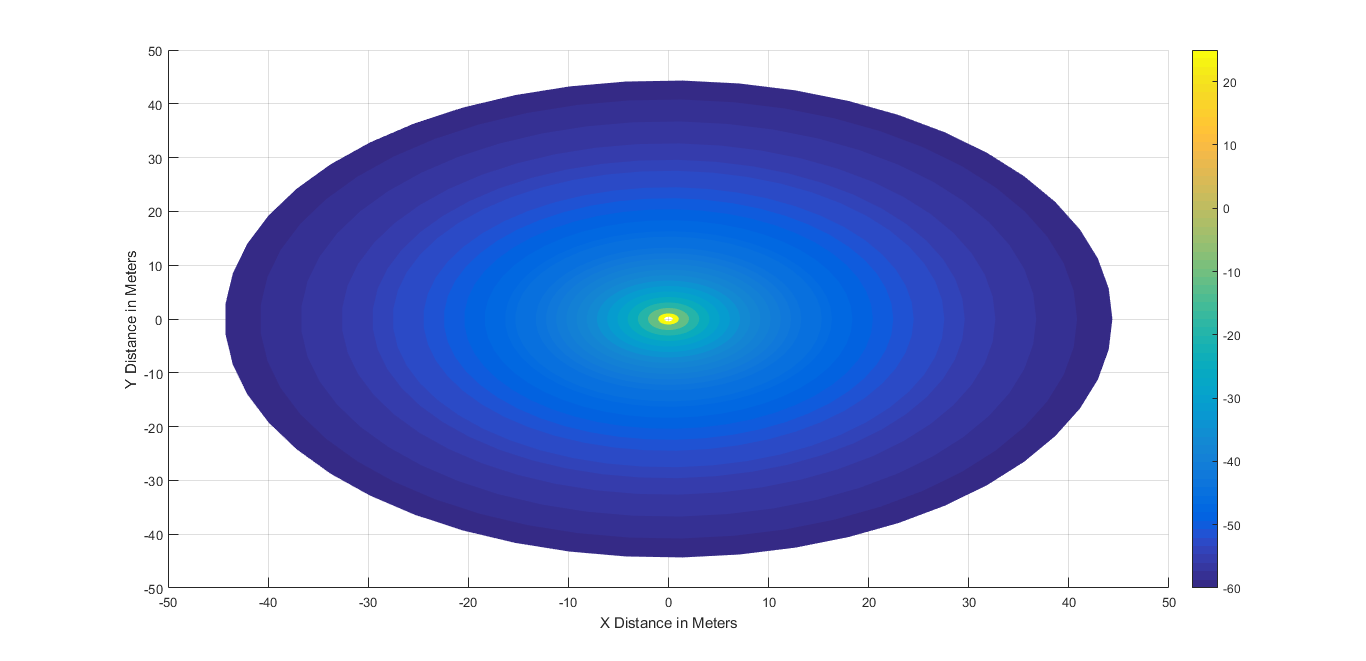
\includegraphics[width=\textwidth]{images/ITU_rm_tv.png}
		\label{subfig:b}
		\caption{}
	\end{subfigure}
\caption{Wi-Fi signal strength plot of ITU indoor model over a 100m spread}
\end{figure*}
The ITU indoor propagation model, also known as ITU model for indoor attenuation, is a radio propagation model that estimates the path loss inside a room or a closed area inside a building delimited by walls of any form. Suitable for appliances designed for indoor use, this model approximates the total path loss an indoor link may experience\cite{31}. Though this model suits best to indoor environments for appliances which use the lower microwave bands around 2.4GHz, it applies to a much wider range typically covering frequency ranges from 900MHz to 5.2GHz.\\ 
The ITU indoor path loss model is expressed as\cite{31}:
\begin{equation}
    L = 20log_{10}f + Nlog_{10}d + P_f(n) - 28
\end{equation}
where,\\
L = the total path loss (dB).\\
f = Frequency of transmission (MHz).\\
d = Distance (m).\\
N = The distance power loss coefficient.\\
n = Number of floors between the transmitter and receiver.\\
P$_f$(n) = the floor loss penetration factor.

The received power is calculated using the expression:
\begin{equation}
    P_r = P_t - (L + R_x + T_x)
\end{equation}
where,\\
P$_r$ = Power received by the receiver (dB)\\
P$_t$ = Power transmitted by AP (dB)\\
R$_x$ = Receiver sensitivity (dB)\\
T$_x$ = Transmitter gain (dB)

The values for the constants used in this work are summarized in Table 4.1. Fig 4.1 shows the pass-loss propagation model of ITU indoor model over a 100m spread. Fig 4.1 (A) shows a 3D view of the radio wave intensity vs distance and Fig 4.1 (B) shows the top view of those intensity levels. Considering the maximum power from a Wi-Fi router and a common receiver sensitivity,which is around -60dB, the signal strengths are thresholded to a high of 25dB and a low of -60dB as shown in the intensity bar plot simulating close to that of a real world. 

\begin{table}[h!]
\centering
\begin{tabular}{c c}
\hline
Variable & Value\\
\hline
f        & 2400 MHz\\
N        & 30\\
n        & 0\\
P$_f$(n) & 11\\
P$_t$    & 23\\
R$_x$    & -60\\
T$_x$    & 6\\
\hline
\end{tabular}
\caption{Table for values used in ITU attenuation model}
\label{table:1}
\end{table}

\subsection{Custom SS model}
\begin{figure*}
\centering
	\begin{subfigure}[b]{\textwidth}
		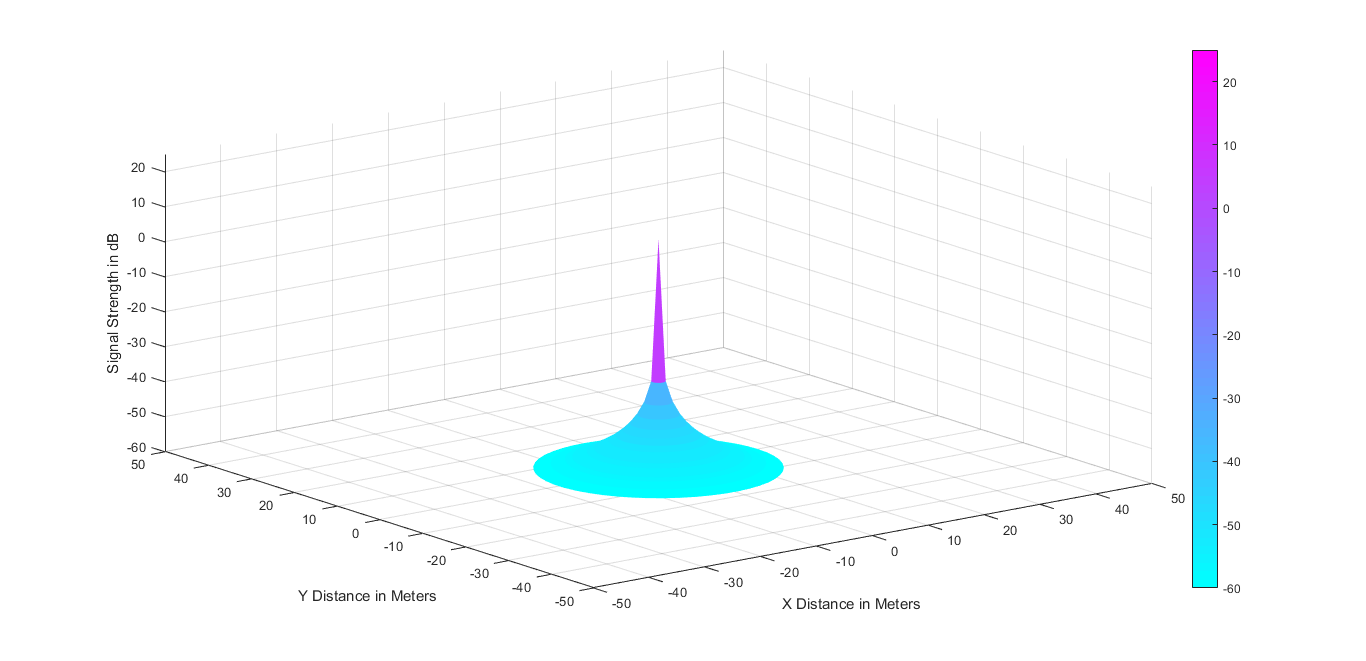
\includegraphics[width=\textwidth]{images/FAL_rm_3d.png}
		\label{subfig:a}
		\caption{}
	\end{subfigure}
    % \vfill
	\begin{subfigure}[b]{\textwidth}
		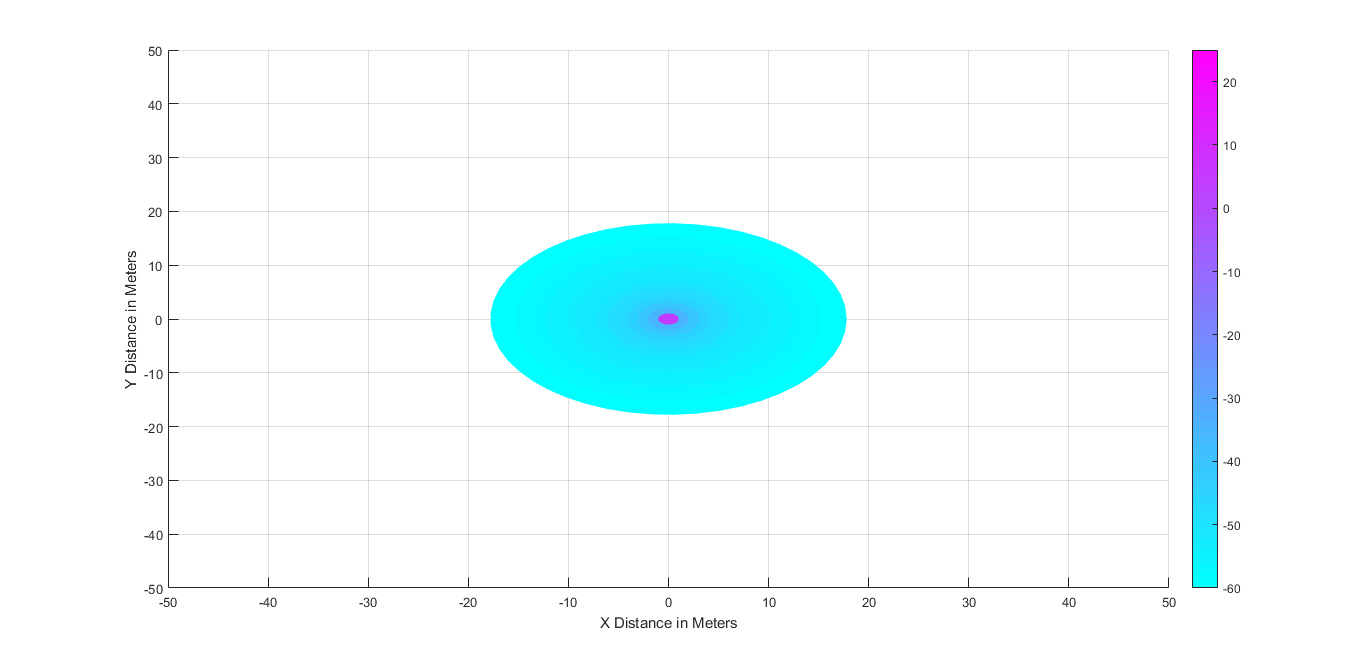
\includegraphics[width=\textwidth]{images/FAL_rm_tv.png}
		\label{subfig:b}
		\caption{}
	\end{subfigure}
\caption{Wi-Fi signal propagation model plot of CSS model over a 100m spread}
\end{figure*}
In order to extensively evaluate the performance of Wi-Coverage, we considered testing in a different radio model with lower signal intensity levels. The CSS model can be mathematically expressed as\cite{30}:
\begin{equation}
    RSS = C - 10nlog_{10}(d) + X_\sigma - 30
\end{equation}
where,\\
RSS = Power received (dB)\\
C = constant\\
n = path-loss exponent\\
X$_\sigma$ = shadow noise modeled as a Gaussian random variable with zero mean and standard deviation $\sigma_{RSS}$

\begin{table}[h!]
\centering
\begin{tabular}{c c}
\hline
Variable & Value\\
\hline
C        & -30\\
n        & 3\\
\hline
\end{tabular}
\caption{Table for values used in CSS propagation model}
\label{table:1}
\end{table}

It can be observed that the signal propagation is much weaker compared to ITU model. A regular receiver cannot sense the AP if more than 17m away.

\section{Maps}
Two maps, free space and office, are created using gazebo to evaluate Wi-Coverage using different performance metrics. Access points are placed at a height of 3m from ground level. The walls of the map are colored on purpose to provide some visual features to RTAB-Map for loop closure detection. Also both maps hold a wooden floor for the same reason and for aesthetics. All maps are unknown to robot while performing exploration and its behaviour is tested in complete autonomous mode.

\begin{figure*}[!h]
    \centering
	\begin{subfigure}[b]{\textwidth}
	    \centering
		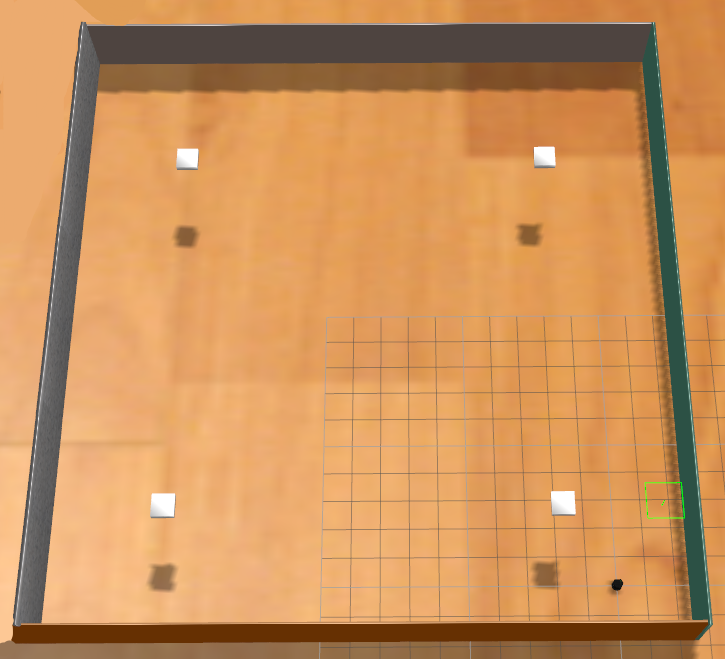
\includegraphics[width=0.5\textwidth]{images/squarespace.png}
		\label{subfig:a}
		\caption{A 30x30m free space with four Wi-Fi routers}
		\vspace{2em}
	\end{subfigure}
    % \vfill
	\begin{subfigure}[b]{\textwidth}
	    \centering
		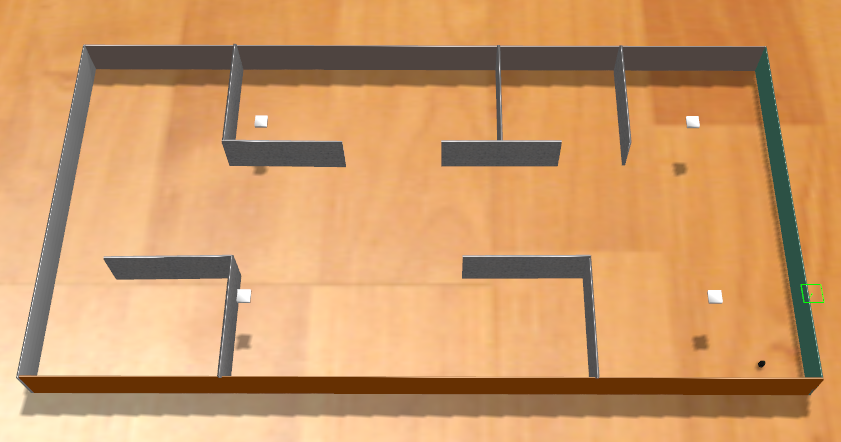
\includegraphics[width=0.75\textwidth]{images/officearea.png}
		\label{subfig:b}
		\caption{An office environment of 60x30m with four APs}
	\end{subfigure}
\caption{Maps created in Gazebo simulator with Wi-Fi APs for evaluating Wi-Coverage}
\end{figure*}

\subsection{Free Space}
Fig 4.3 (A) shows a square area of 30x30m free space powered with four simulated APs shown in white cubes.  Figs 4.4 and 4.5 shows the radio waves propagation in the free space map with four APs. The peaks represent the location of the APs. Fig 4.4 (A) is the SS vs distance plot for ITU indoor model. It is worth noting that all APs have an overlap of their signals with each other. This also implies that the robot would sense atleast one or in this case all four APs from any location in the map. Fig 4.4(B) is a top view of the previous figure. On contrary, in case of CSS model, there exist deaf spots or the places where none of the APs can be sensed. It is useful in understanding the algorithm's take on deaf spots. Also there is no overlap of signals between APs cross opposite to each other. 

\begin{figure*}[!h]
\centering
	\begin{subfigure}[b]{0.75\textwidth}
		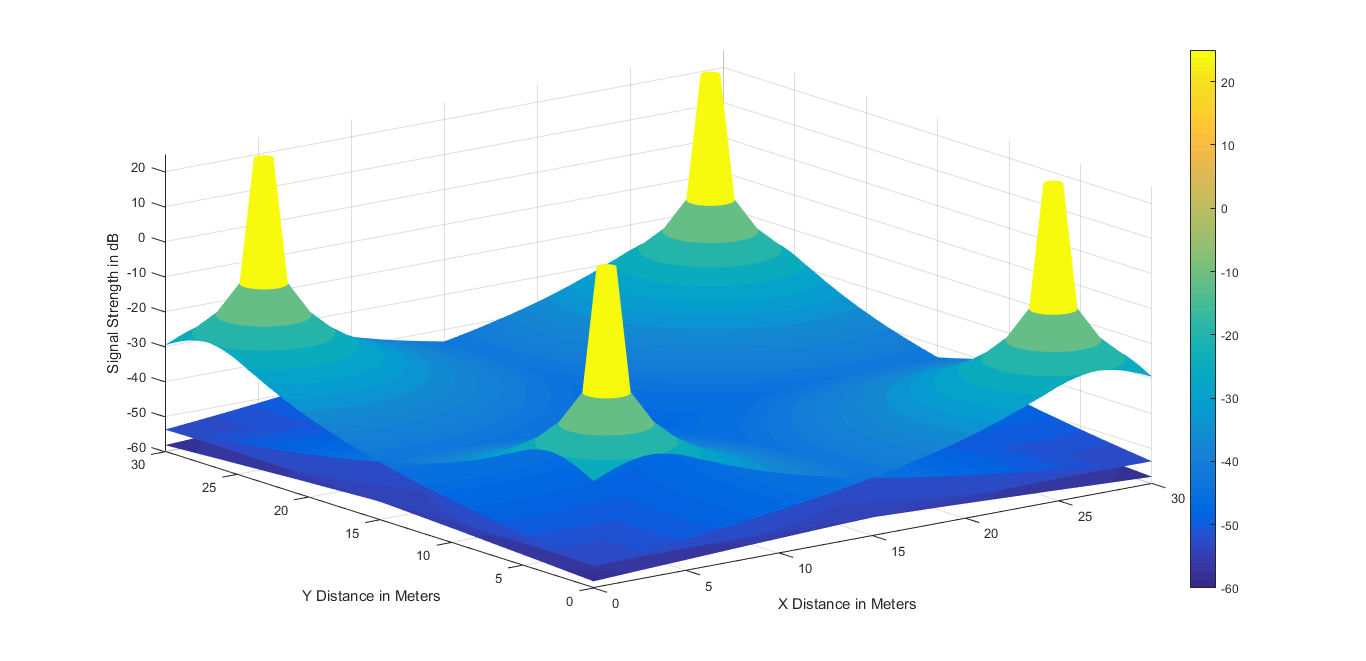
\includegraphics[width=\textwidth]{images/ITU_30x30_3d.png}
		\label{subfig:a}
		\caption{}
	\end{subfigure}
    % \vfill
	\begin{subfigure}[b]{0.75\textwidth}
		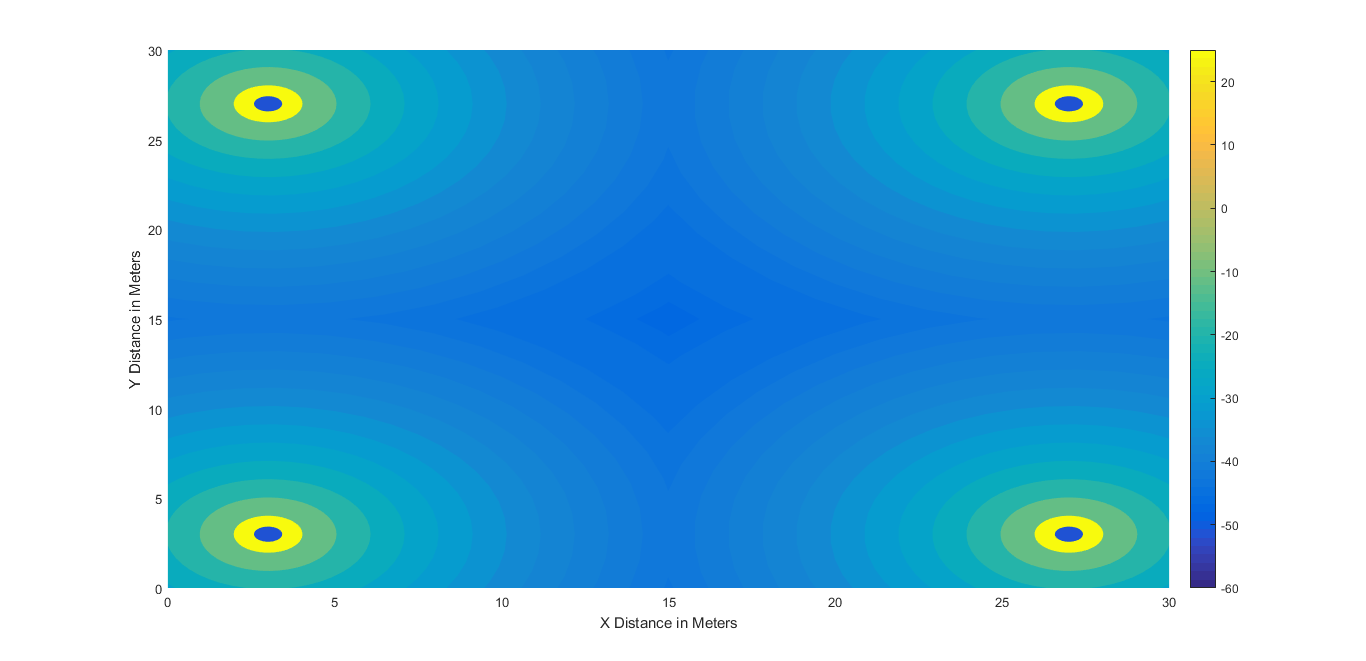
\includegraphics[width=\textwidth]{images/ITU_30x30_tv.png}
		\label{subfig:b}
		\caption{}
	\end{subfigure}
\caption{ITU propagation model in free space map with four APs. The bar chart indicates the intensity in dB}
\end{figure*}

% Fig 4.5 shows the propagation model for ITU indoor model which is much closer to reality. It has an overlap between all four APs in case of the free space map.
\begin{figure*}[!h]
\centering
	\begin{subfigure}[b]{0.75\textwidth}
		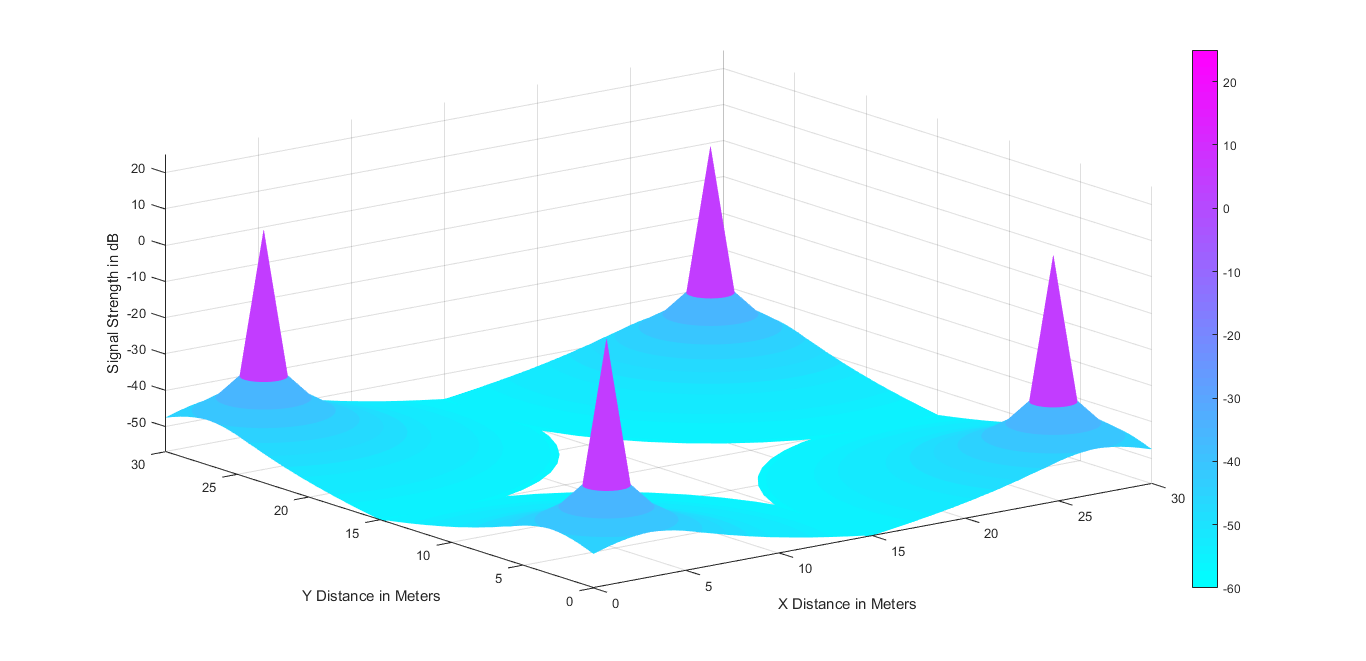
\includegraphics[width=\textwidth]{images/FAL_30x30_3d.png}
		\label{subfig:a}
		\caption{}
	\end{subfigure}
    % \vfill
	\begin{subfigure}[b]{0.75\textwidth}
		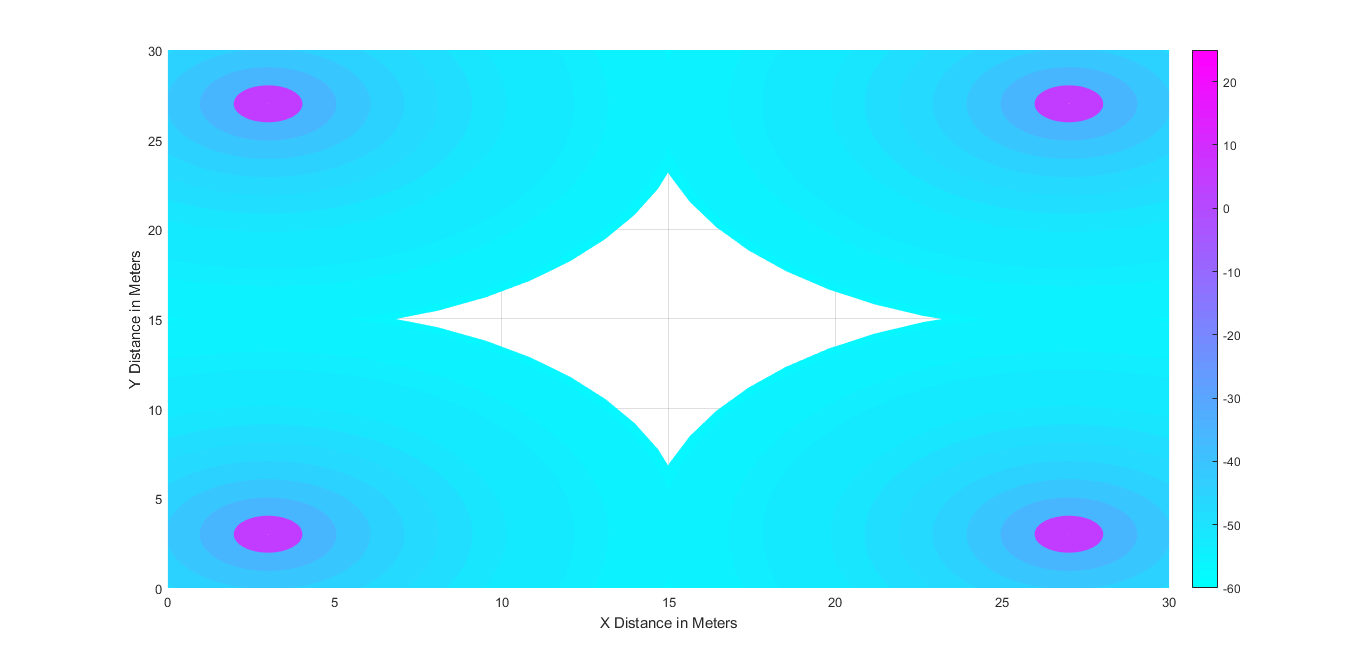
\includegraphics[width=\textwidth]{images/FAL_30x30_tv.png}
		\label{subfig:b}
		\caption{}
	\end{subfigure}
\caption{CSS propagation model in free space map with four APs. The bar chart indicates the intensity in dB}
\end{figure*}

\begin{figure}
    \centering
    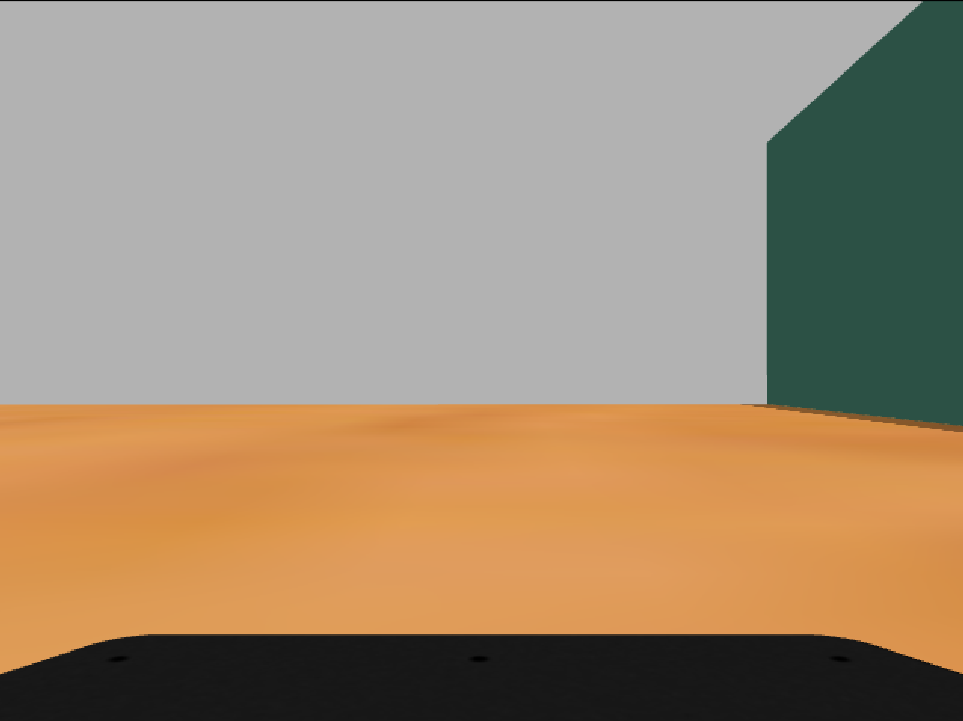
\includegraphics[width=0.5\textwidth]{images/robotview.png}
    \caption{The robots view at the start of the exploration.}
    \label{fig:freespace}
\end{figure}

\subsection{Office Space}
Fig 4.3 (B) represents a typical office space with cubicles and inlets. rectangle hall with obstacles resembling real world environment. This environment also has the same AP location configuration as that of the previous one.

\section{Coverage Results}
Simulation results are obtained for each map shown in fig 4.3 using a single robot. As mentioned before, no prior information about the environment including AP locations are provided to the robot. Maps are loaded and displayed in Gazebo for visualization and debugging purposes. Fig 4.6 represent the robots view of the environment at the start of exploration. Robot can be started at any location to achieve full coverage. Fifteen simulations are run in each environment with two different Wi-Fi signal strength models: ITU indoor model and custom signal strength(CSS) model. Results for coverage vs time contain standard deviations for each method and environment tested in. The time units used in results is real-time seconds obtained from ROS time.

\subsection{Robot Trajectories}
Robot trajectories are plotted for each method in both the SS models to present the robots systematic behaviour. All Wi-Coverage trajectories plotted are color coded. Each color represent an AP and its associated robot trajectory. Smaller points represent the frontier poses picked by the robot and lines represent the robot trajectory. The color of the line represent the robots exploration in the corresponding AP cluster. Each cluster has its own color same as that of its AP and a change in the line color implies that the robot has completely explored the current cluster and is moving to the next best cluster as per the algorithm. The bigger color dots in the graphs show that the robot has entered a different AP cluster while exploring the current cluster. Color of the dot represent the AP cluster it realizes and associates all new frontiers to that cluster (see chapter 3). Also all robots start from the origin which is at bottom right corner. The following is a legend explaining the representations involved in the trajectory plots.

\begin{figure}[!h]
    \centering
    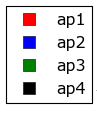
\includegraphics[width=0.2\textwidth]{images/legend.png}
    \caption{A legend for robot trajectory plots of Wi-Coverage}
    \label{fig:freespace}
\end{figure}

\subsubsection{Free Space Robot Trajectories}

\begin{figure*}[!h]
\centering
	\begin{subfigure}[b]{\textwidth}
	    \centering
		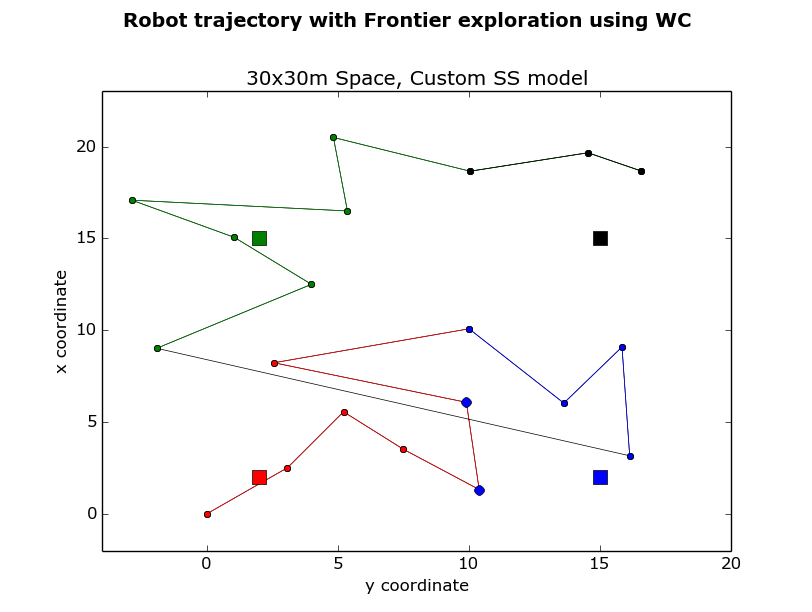
\includegraphics[width=0.95\textwidth]{images/traj_cm_30x30.png}
		\label{subfig:a}
		\caption{CSS model}
	\end{subfigure}
    % \vfill
	\begin{subfigure}[b]{\textwidth}
	    \centering
		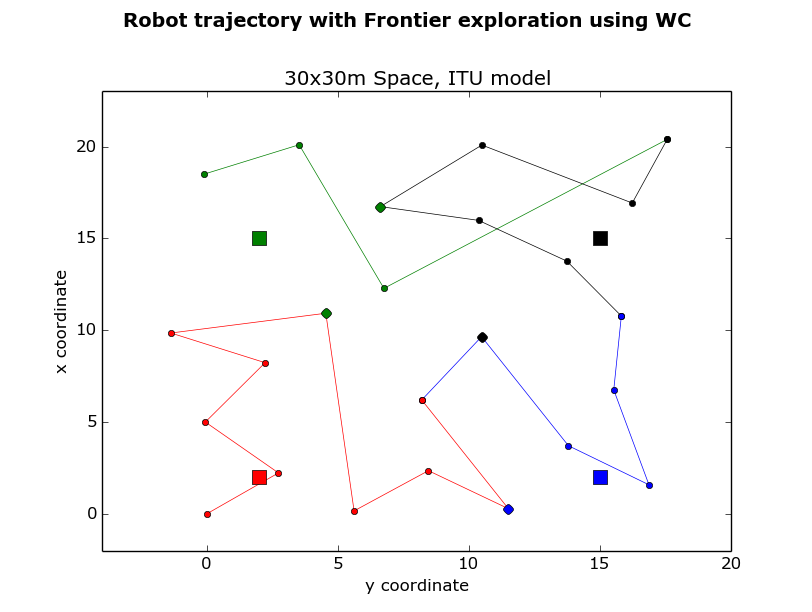
\includegraphics[width=0.95\textwidth]{images/30x30_itu_traj_final.png}
		\label{subfig:b}
		\caption{ITU model}
	\end{subfigure}
\caption{Robot trajectories in free space map}
\end{figure*}

This environment is created relatively simple with no obstacles which will help evaluate the free form of Wi-Coverage in performing online clustering. It also helps evaluating the robots movement when compared to other methods. Fig 4.8 and 4.9 show the plots of Darwin's trajectory in free space map using Wi-Coverage and Information gain based frontier exploration. In case of Wi-Coverage, there are always a finite set of possible trajectories which can be helpful in predicting robots next move if necessary. The trajectories shown is one such possibility which we recorded while experimenting. They keep varying based on the sensor's accuracy and varying signal strengths especially in case of CSS model due to a shadow noise added in the propagation model. 

\par Fig 4.8 (A) shows a trajectory in CSS model with four APs. The robot starts with cluster AP1 and identifies two frontiers cells in cluster AP2. It can be noticed that the robot chose the last red pose (6.3, 4.2) which completely explores the cluster AP1 and moves ahead to cluster AP2. Later it moves to cluster AP3 as an unexplored frontier opened previously by the robot while exploring cluster AP1. The robot then completely explores cluster AP3 and finally its successful exploration comes to an end after exhausting all frontiers of cluster AP4. Similarly in the ITU model due to a bigger overlap, the robot has opened frontiers from all the unexplored clusters and sorts them. This information is later used to select the next best cluster based on the information gains of the cluster's unexplored frontiers. Robot trajectory for frontier exploration using optimal information gain policy is shown in Fig 4.9. It can be noticed that the breadths and depths of the search are not well defined and is highly unpredictable.

\begin{figure}[!b]
    \centering
    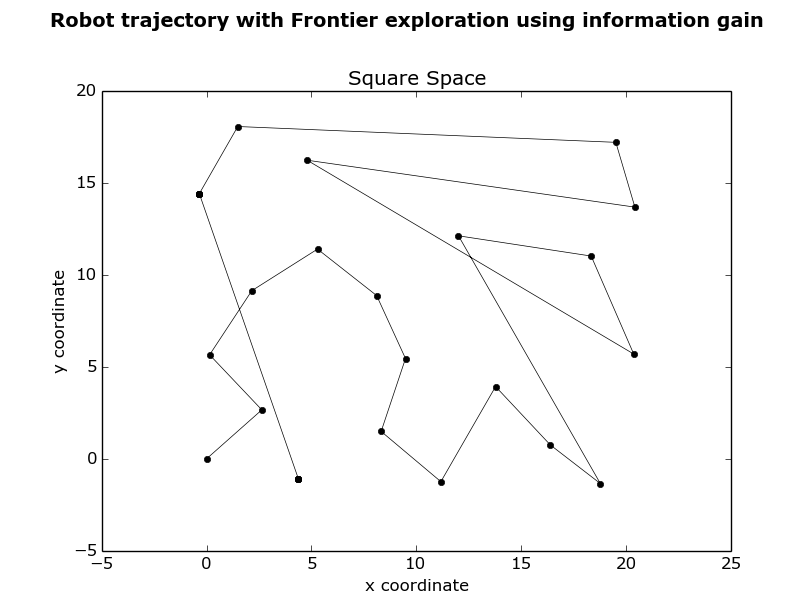
\includegraphics[width=0.75\textwidth]{images/infosquare.png}
    \caption{Robot trajectory in free space map using Information gain based exploration}
    \label{fig:info}
\end{figure}

\subsubsection{Office Space Robot Trajectories}
Office map is a relatively complex environment that simulates real world obstacles like walls and inlets like cubicles. This map is spread across an area of 60x30m and powered by four APs capable of simulating two radio signal propagation models for testing. Robot trajectories for both SS model configurations are shown in the Fig 4.10. Wi-Coverage helps achieve a systematic exploration. From the trajectory graphs it can clearly observed that, the robot finishes exploring the cubicles under an AP completely and later moves to the other cubicles thereby completely covering the entire space in a systematic, breadth and depth defined like search. On the other hand information gain method made the robot move along the hallway and later cover the left over cubical spaces increasing the robot trial and hence coverage time. This can particularly be a disadvantage when exploring offices with long hallways. The difference in propagation model has not effected Wi-Coverage much, since in deaf spots the robot continuous to explore based on information gain until it senses an AP which triggers Wi-Coverage.    

\begin{figure*}[!h]
\centering
	\begin{subfigure}[b]{\textwidth}
	    \centering
		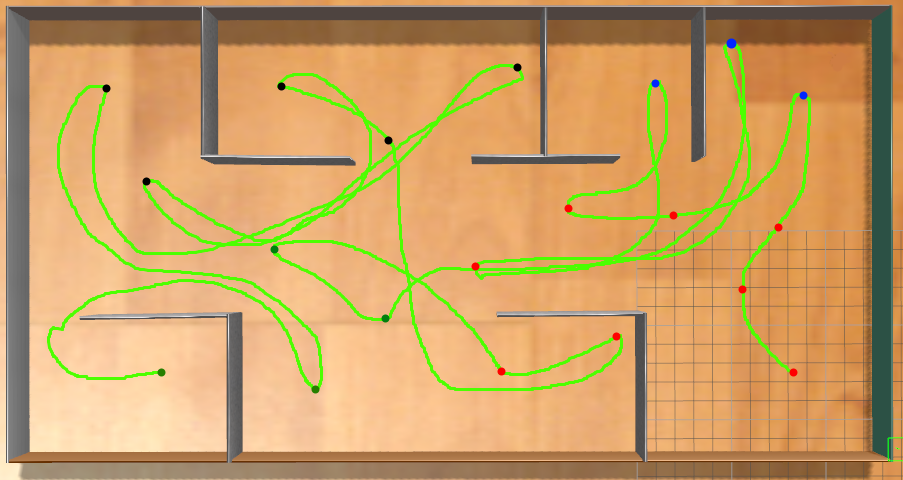
\includegraphics[width=0.95\textwidth]{images/trajitu.png}
		\label{subfig:a}
		\caption{CSS model}
		\vspace{2em}
	\end{subfigure}
    % \vfill
	\begin{subfigure}[b]{\textwidth}
	    \centering
		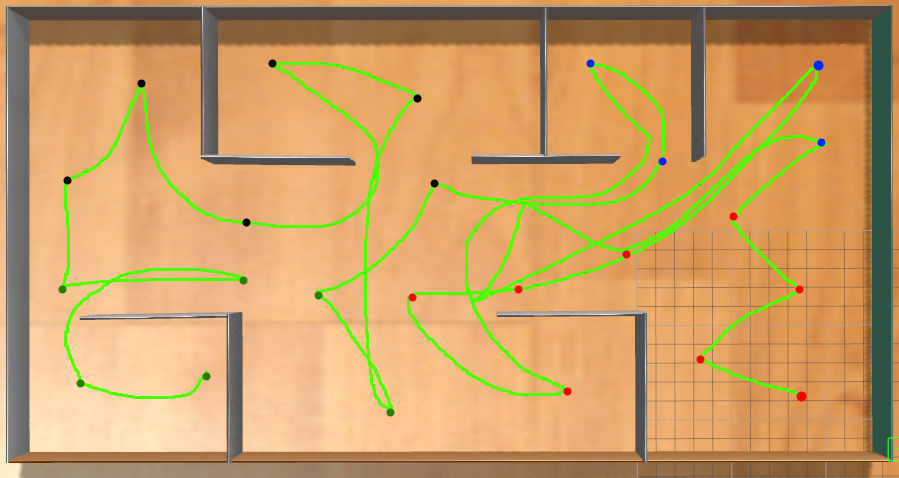
\includegraphics[width=0.95\textwidth]{images/trajcss.png}
		\label{subfig:b}
		\caption{ITU model}
	\end{subfigure}
\caption{Robot trajectories in the office space}
\end{figure*}

\begin{figure}[!h]
    \centering
    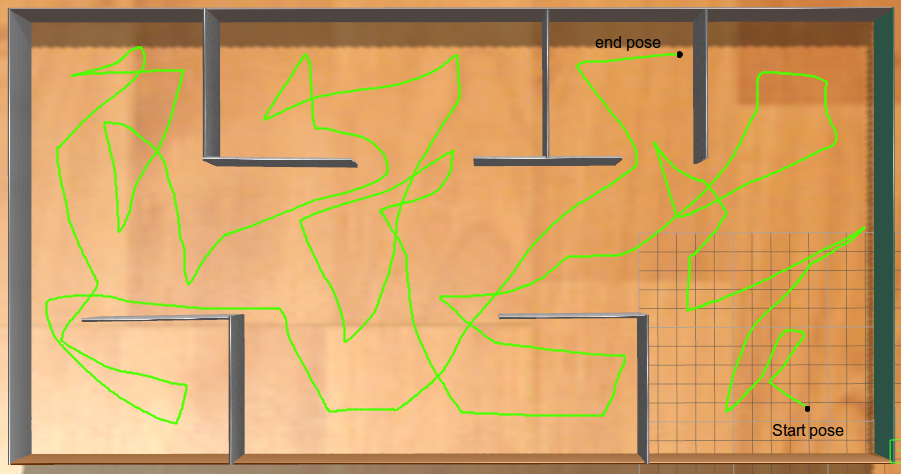
\includegraphics[width=0.75\textwidth]{images/trajig1.png}
    \caption{Robot trajectory in office space using information gain based exploration.}
    \label{fig:info}
\end{figure}

\subsection{Coverage Area vs Time}
Both the methods compared, explore completely any given space since both methods use frontier exploration. The only difference is in the method of allocating frontiers. Since exploration is a time sensitive problem, coverage time is an important metric to be considered for evaluation. 

\subsubsection{Free Space}

Fig 4.11 (A) plots the time taken to completely cover the environment in free space map with two propagation models: ITU model and CSS model. Wi-Coverage is compared to optimal information gain policy in both models. Minimum, Maximum and average times taken to explore completely are shown in the plot. The numbers on the top of the bars show the average time for that method. Fig 4.11(B) shows a plot of percentage coverage area vs time. Time taken to cover every quarter percentage area of total space is plotted. Information gain based exploration has the best average time of 821.32 secs followed closely by Wi-Coverage strategy with also a 100\% coverage in an average time of 875.86 and 904.32 secs in CSS and ITU models respectively. 

\begin{figure*}[!h]
\centering
	\begin{subfigure}[b]{0.75\textwidth}
		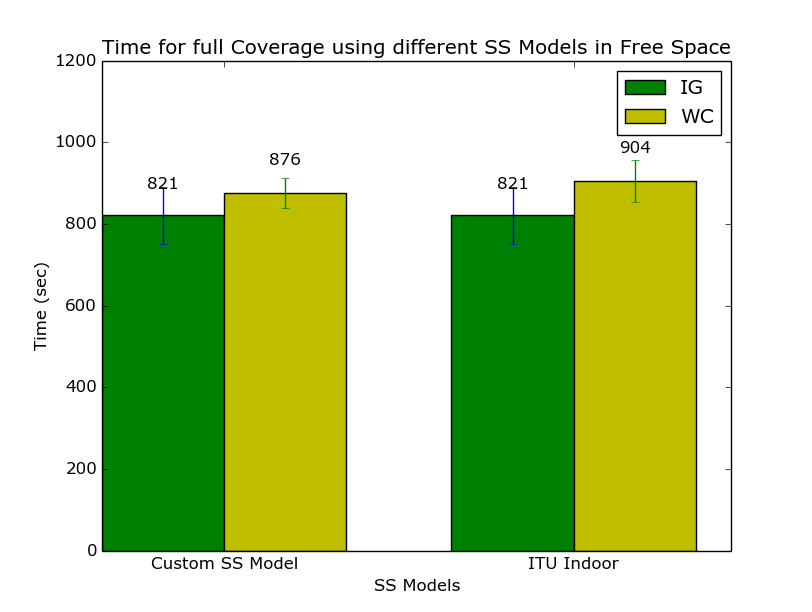
\includegraphics[width=\textwidth]{images/full_ct.png}
		\label{subfig:a}
		\caption{Free Space}
	\end{subfigure}
    % \vfill
	\begin{subfigure}[b]{0.75\textwidth}
		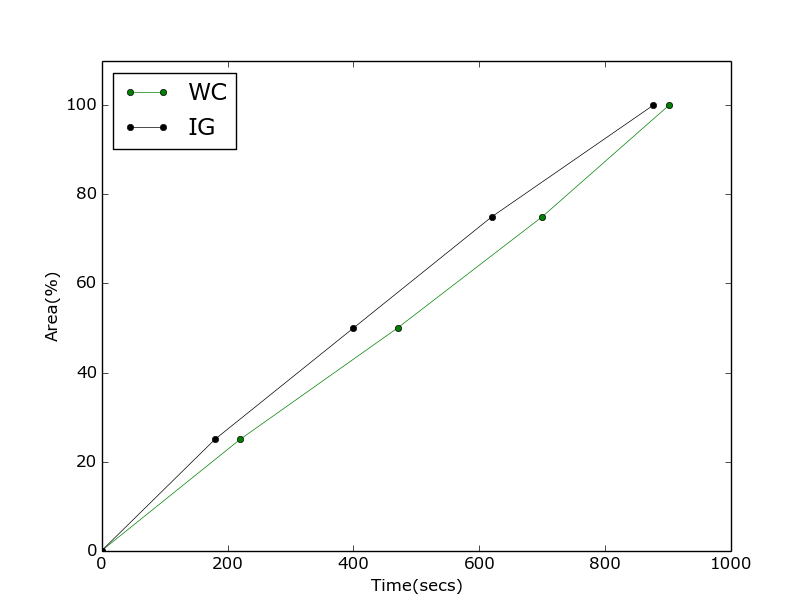
\includegraphics[width=\textwidth]{images/freespace.png}
		\label{subfig:b}
		\caption{Office Space}
	\end{subfigure}
\caption{Percentage Coverage Area vs time in free space}
\end{figure*}

\subsubsection{Office Space}
The coverage results for office environment are plotted in Fig 4.12. Fig 4.11(A) shows the plot of full coverage time for both methods in different SS models. Information gain based exploration explored the complete space in an average time of 1874.56 secs. Wi-Coverage in CSS model achieves this in an average time of 1892.48 secs which is closely followed by Wi-Coverage in ITU indoor model completing the entire space in 1902.12 secs. The coverage results of Wi-Coverage are pretty comparable to the information gain approach. Fig 4.12(B) shows the percentage area covered vs time. It is clear from the results that Wi-Coverage trails very close to the gold standard of frontier exploration. Fig 4.12 plots the percentage covered area with time for Information gain based exploration and Wi-Coverage in ITU indoor model. This graph explains that information gain based exploration has a quicker percentage of area covered at the beginning since it mostly explores the hallway first. But at the end, the coverage time increases due to longer trails in order to reach unexplored patches. On contrary, Wi-Coverage  almost had a linear relationship between percent area covered and time except at some places where we observe a dip. These minor dips occur due to the rejection of most optimal frontier in order to visit already queued frontier of the same cluster which is the basis of Wi-Coverage: to first exhaust the frontiers of current cluster before moving to the next. But this is almost compensated at the end of the exploration since the robot has to make smaller trails to finish the remaining unexplored space.  

\begin{figure*}[!h]
\centering
	\begin{subfigure}[b]{0.75\textwidth}
		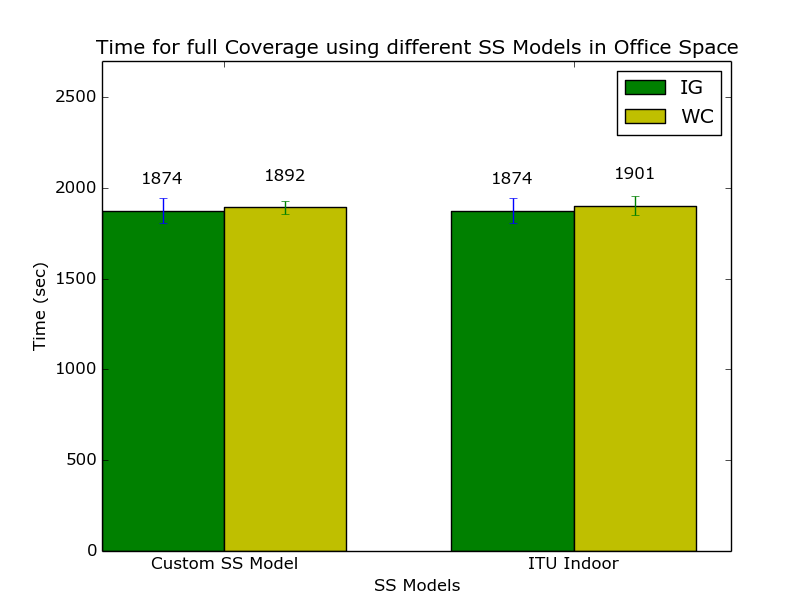
\includegraphics[width=\textwidth]{images/bargoffice.png}
		\label{subfig:a}
		\caption{Free Space}
	\end{subfigure}
    % \vfill
	\begin{subfigure}[b]{0.75\textwidth}
		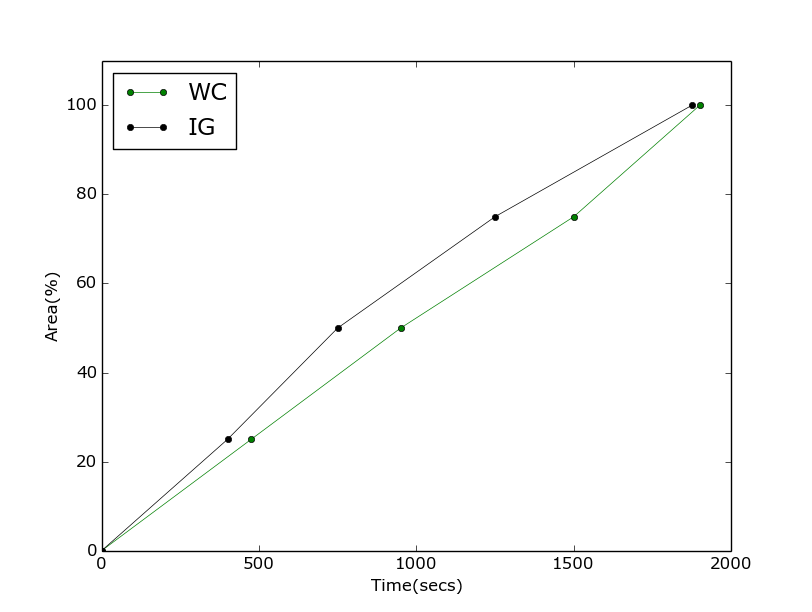
\includegraphics[width=\textwidth]{images/60x30office.png}
		\label{subfig:b}
		\caption{Office Space}
	\end{subfigure}
\caption{Percentage Coverage Area vs time in office space}
\end{figure*}

\section{Issues}
The primary reason is the exploration strategy, which decides, which sensor the robot adorns. As discussed in the previous chapters, there are a number of approaches for autonomous robot exploration. In this work we used RGB-D data from a vision sensor which is a Kinect Xbox 360 and a visual slam package RTAB-Map to perform autonomous exploration using a frontier based approach. This setup used is common in all the experiments and the following issues and solutions are particular to the sensor and packages(See Chapter 3) used in this work, unless explicitly specified.  

\subsection{Glass and reflective surfaces}

\begin{figure}
    \centering
    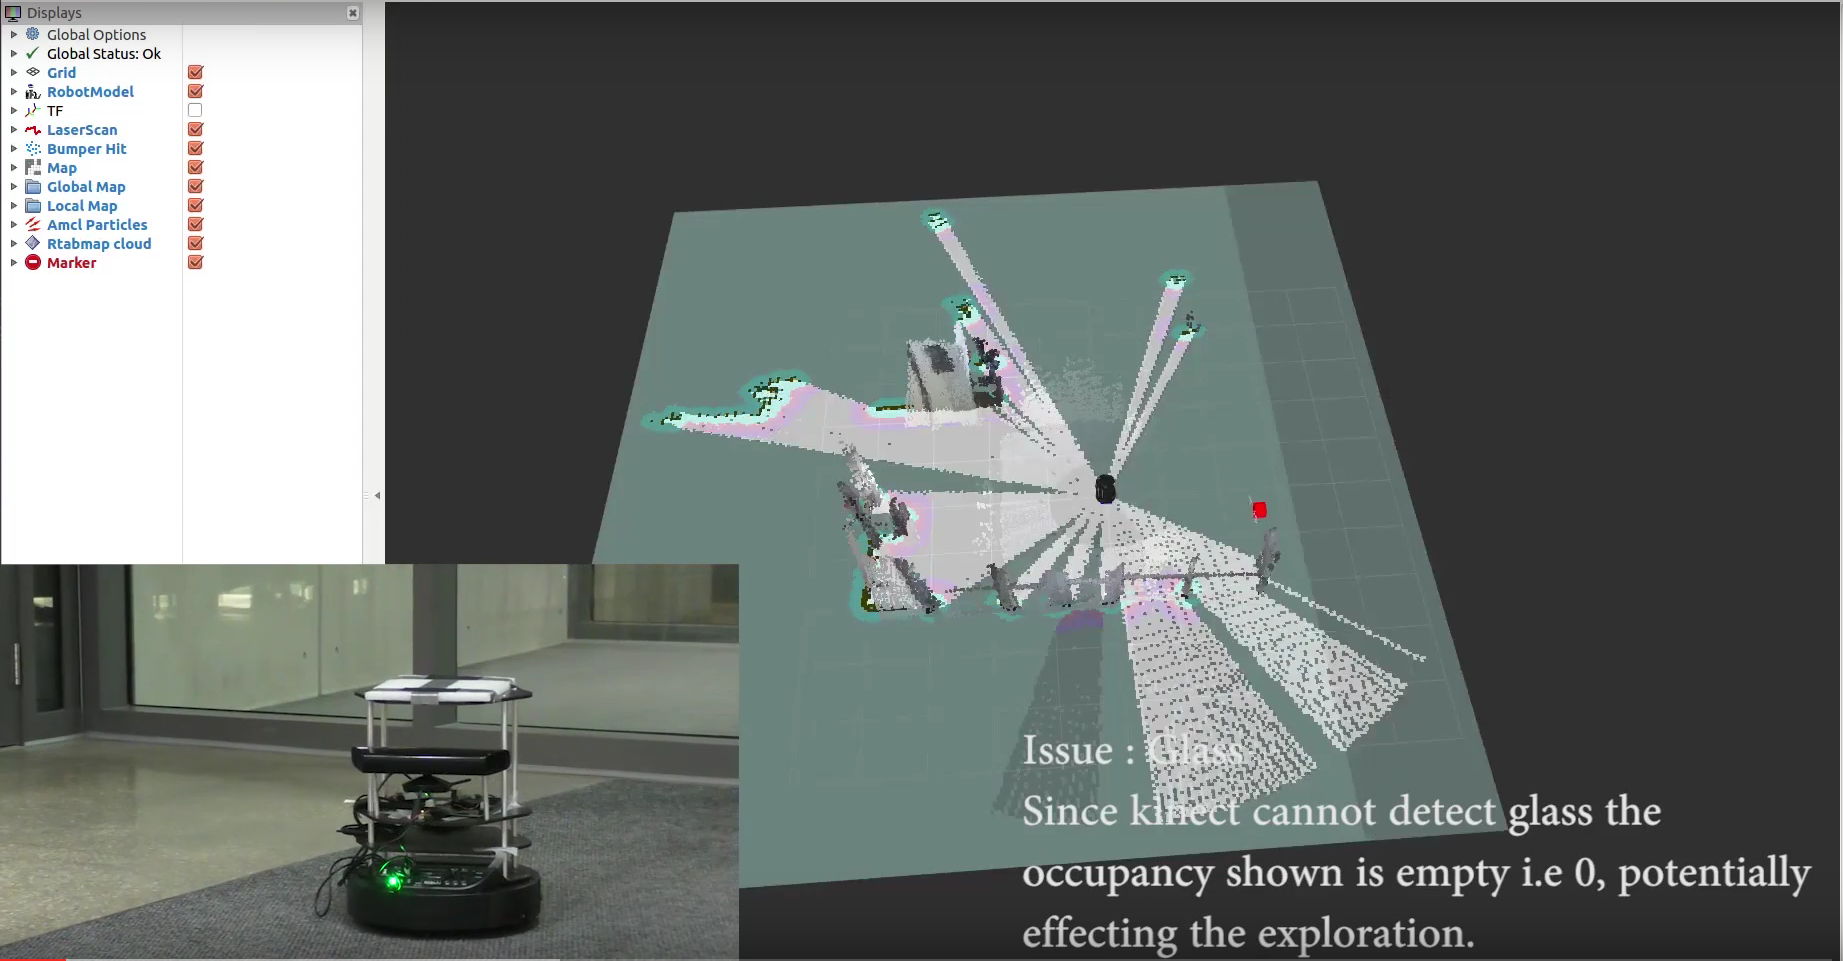
\includegraphics[width=0.75\textwidth]{images/Glass_ppt.png}    
    \caption{Sensor scan representing failed detection of a transparent(Glass) surface}
    \label{fig:my_label}
\end{figure}

Walls and windows made of glass can be found in almost any urban setting such as airports, malls, offices and even some homes. 
Light sensors like stereo cameras or lidars are incapable of detecting such transparent and reflective surfaces. This is a common problem faced in any exploration or mapping application. Figure 4.14 above shows an experiment (snapshot from Rviz) conducted in Davis Hall, University at Buffalo. The robot performs a sensor sweep to identify frontiers and assumes an empty space beyond the glass doors which was later accounted for containing frontiers and the robot bumps into the glass. Similarly, when a reflective surface is confronted by such sensors, the point cloud would contain the reflection thereby effecting the algorithm's judgment.

\lhead{\emph{Issues}}
\textbf{Solution}:
A traditional and probably the only simple solution is to use a sonar. The sonar is swept across the environment along with the vision sensor and the evidence grid is updated by filtering such specular reflections and transparent obstacles such as glass by limiting the range to that of sonar. The disadvantage in this approach is the addition of a new equipment to the robot making it expensive and bulky.

\subsection{Sensor uncertainty}
When frontiers detected are false or redundant, explored space is re-explored increasing the coverage time  and thereby reducing the efficiency. This happens when the sensor model estimate is erroneous in a portion of the map explored and calculations are performed on it without pre-processing or filtering. For example, when a sensor sweep is performed and the sensor is uncertain about the occupancy of a grid cell, corresponding evidence grid is erroneous thereby effecting all the consequent stages in the algorithm. Fig. 4.15 below shows such a scenario. The sensor model was unsure in classifying some grid cells to empty or occupied hence resulting in an unknown grid cell which in fact was an empty cell. Later with this occupancy grid, the next best point was formulated to be this false unknown cell lying in between empty cells which were already mapped and added to the point cloud. This redundant move increased the full coverage time of the exploration making it inefficient. 

\begin{figure}
    \centering
    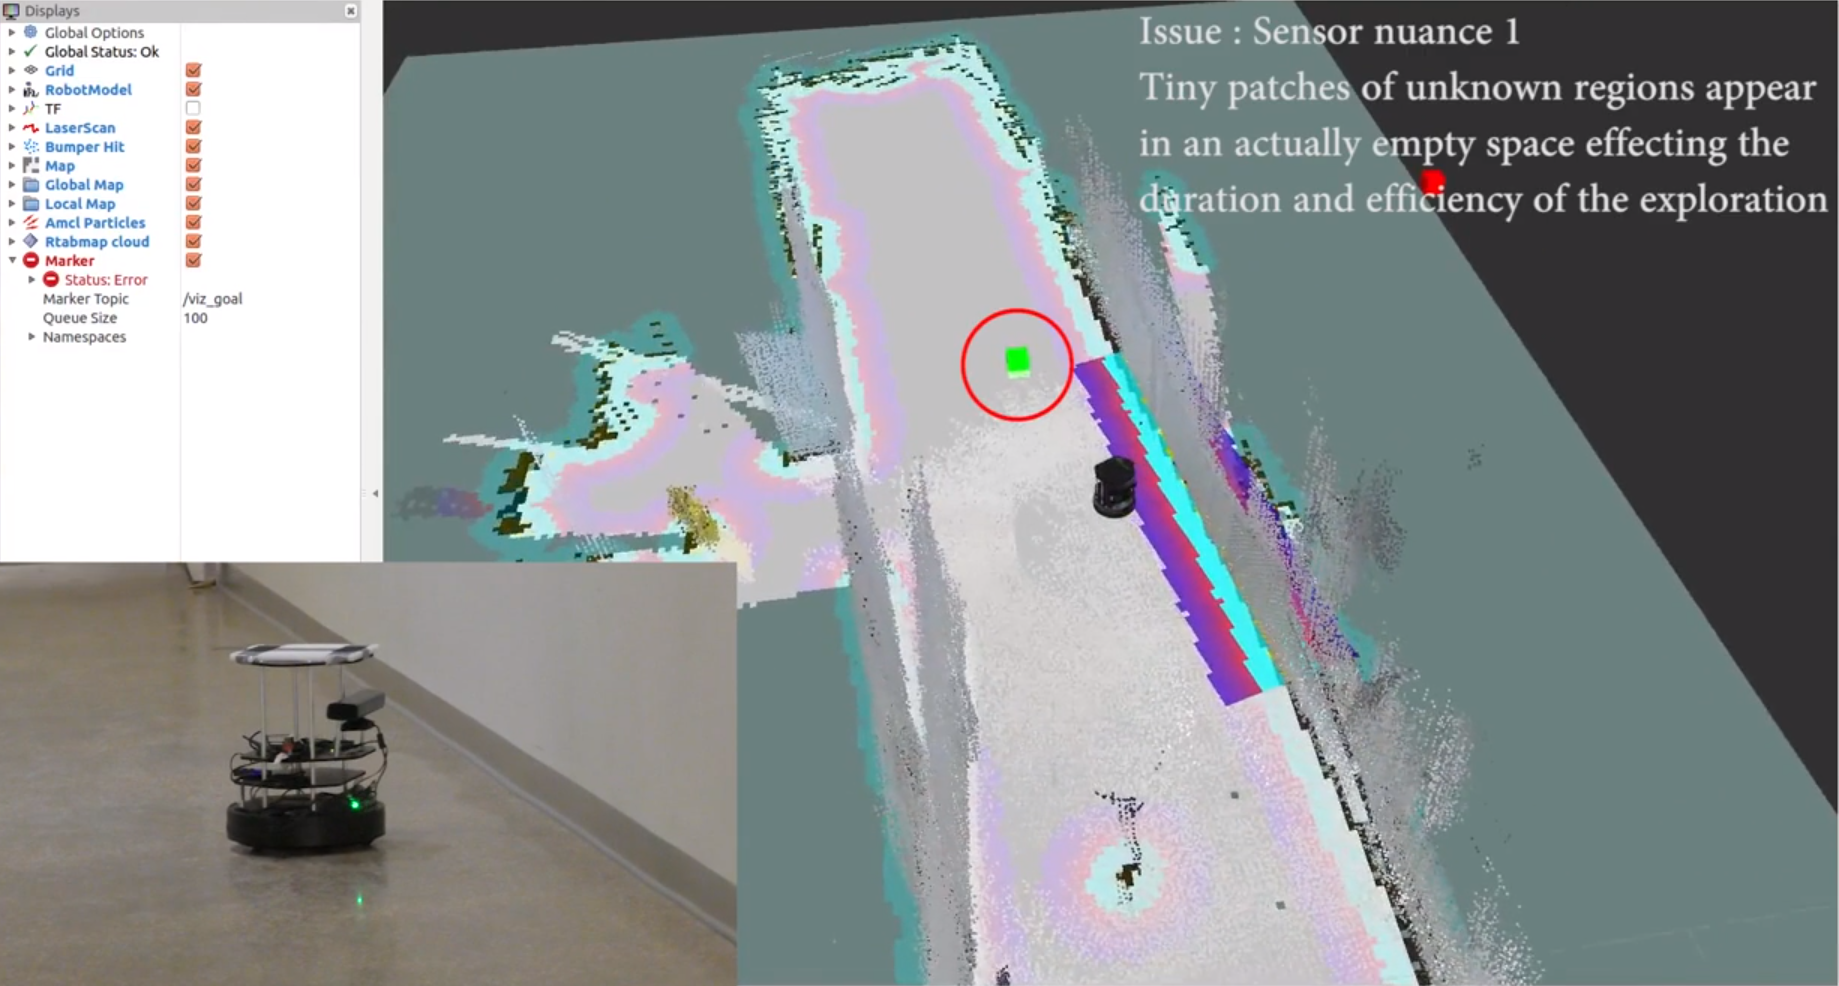
\includegraphics[width=0.75\textwidth]{images/falsefrontier.png}
    \caption{A false frontier detected in an explored empty space}
    \label{fig:my_label}
\end{figure}

\textbf{Solutions}: 
This issue can be overcomed using two approaches,
\begin{itemize}
    \item \textbf{Custom resolution} : One of the approach to overcome redundant frontiers is to increase the resolution of the occupancy grid generated. In general, this is a parameter in the mapping package which can be tweaked. If not, a custom occupancy grid(bigger than the original) is to be generated with a policy that determines the final occupancy of the cell based on the threshold count of type of cells in the original grid. For example, if the grid has 98\% of empty cells and 2\% of unknown cells, it is safe to consider the occupancy of the cell in the new resolution grid as empty which eliminates spurious frontiers in already mapped areas.
    \item \textbf{Post processing} : Another approach would be to post process the frontiers identified and threshold them such that only valid frontiers are queued. Again, the thresholding can be performed based on the neighbouring grid cells irrespective of the resolution of the current occupancy grid.  
\end{itemize}

\subsection{Dynamic environments}
Obstacles moving in the environment could effect identifying frontiers turning them out as false ones. Fig 4.16 represent an exploration trial wherein at one of the sensor sweeps a door was opened and tiny points from the sensor are added to the point cloud. Later the door was closed and as expected the next best goal was inside the room since the information gain around the point was large. The robot performs a failed attempt to move to the goal position since the path was blocked and rejects the frontier after it reaches the maximum times of attempts. 

\textbf{Solution}:
Most implementations follow the traditional approach of having a maximum number of attempts the robot can have in reaching its next best position in the environment. Having reached the maximum number of tries, the respective frontier is deemed inaccessible and the robot attempts to reach the next best frontier in the queue. Though this practice works well, the exploration time would drastically increase in a clustered environment especially with decent sized robots whose footprint matters such as of a Turtlebot. As mentioned above, post processing the frontiers can help eliminate such futile attempts to reach frontiers which creep into the point cloud due to the dynamicity in the environment saving the time for exploration. 
\begin{figure*}
    \begin{subfigure}[b]{0.498\textwidth}
		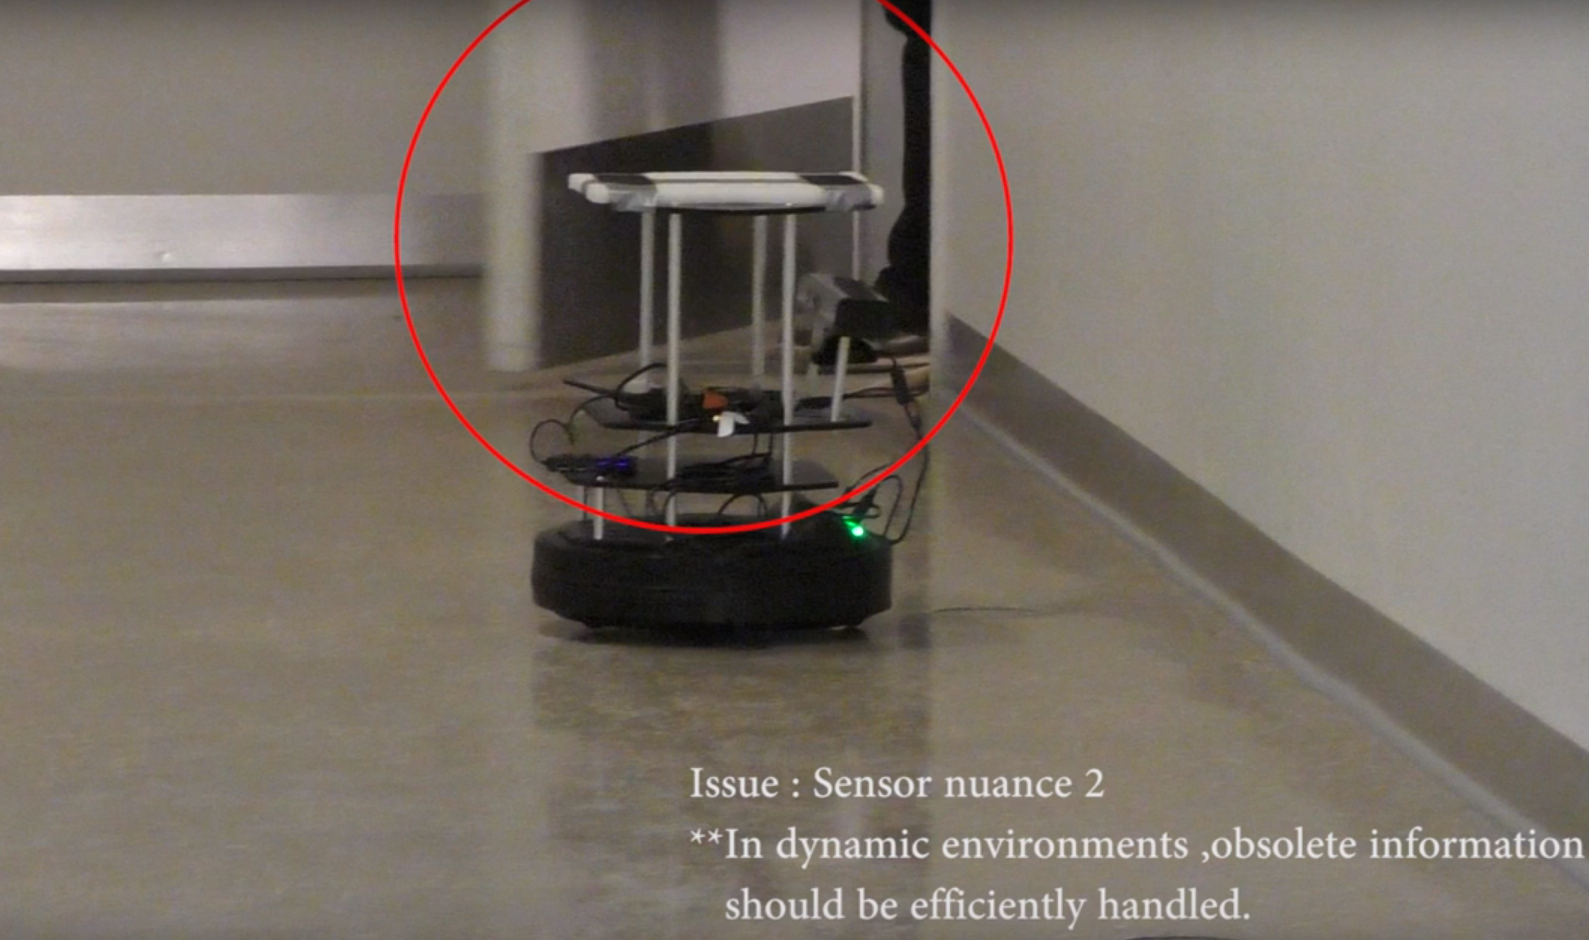
\includegraphics[width=\textwidth, height=0.6\textwidth]{images/maprate.png}
		\label{subfig:a}
		\caption{}
	\end{subfigure}
	\begin{subfigure}[b]{0.498\textwidth}
		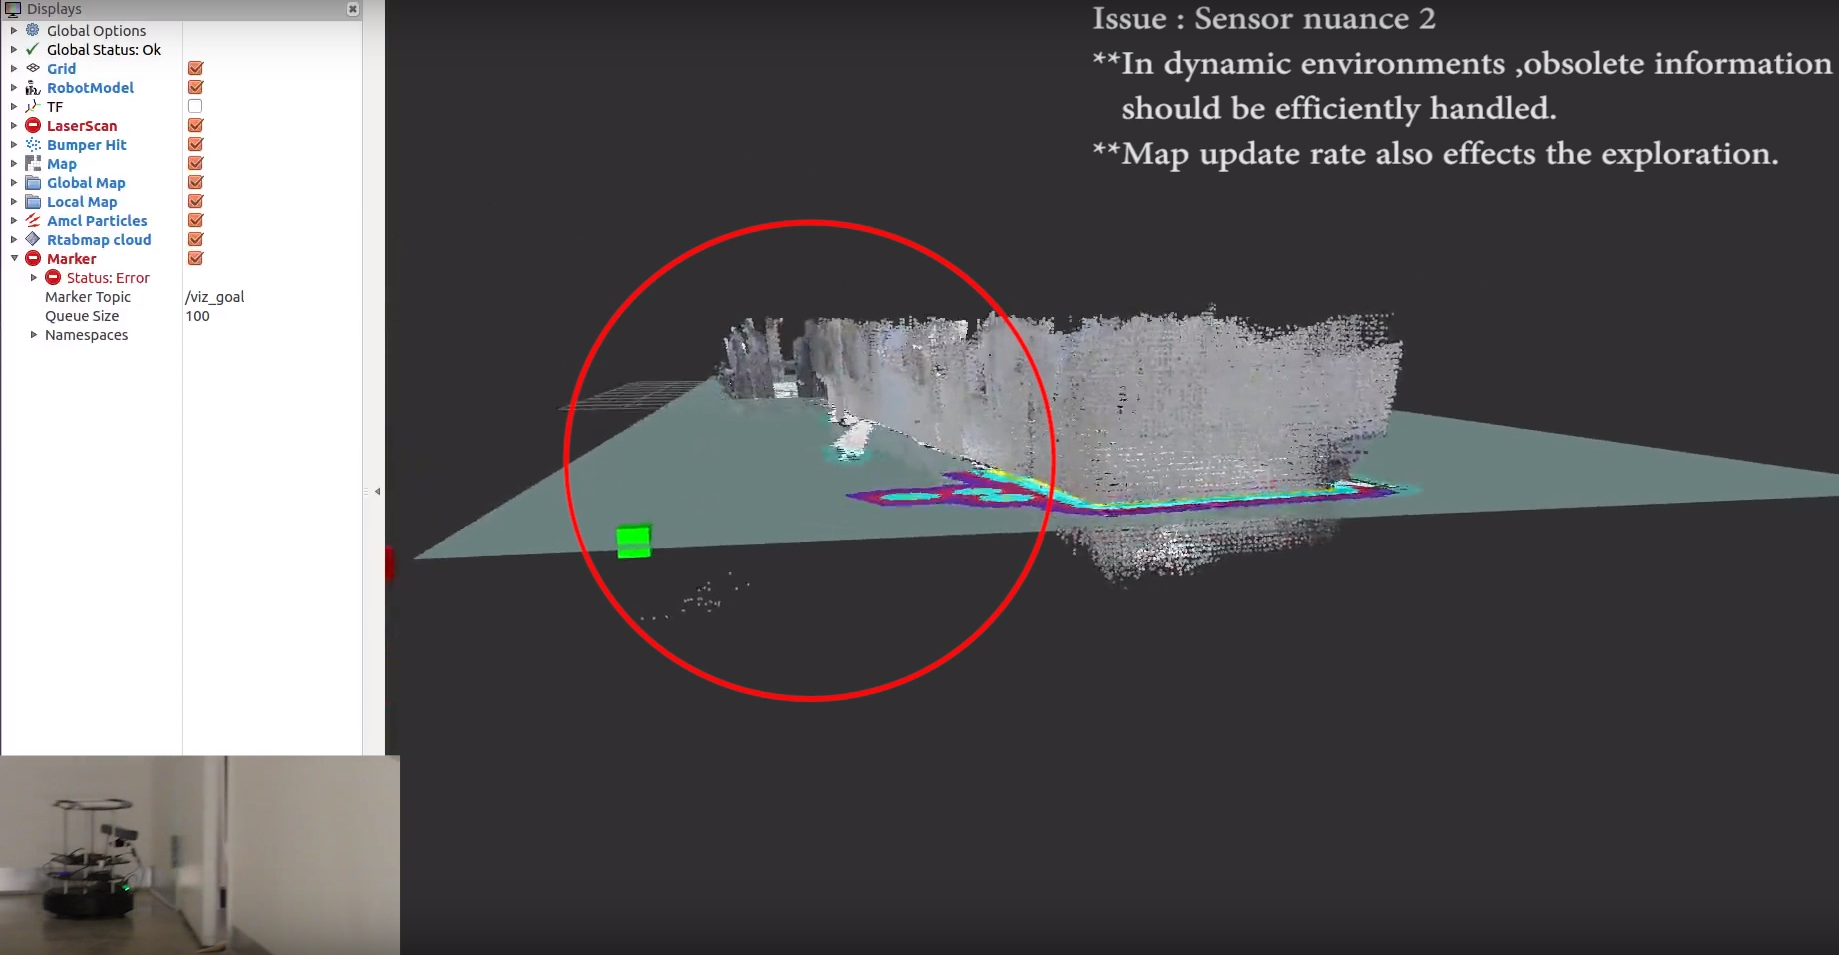
\includegraphics[width=\textwidth, height=0.6\textwidth]{images/map2.png}
		\label{subfig:b}
		\caption{}
	\end{subfigure}
\caption{(A) Image shows a dynamic environment: Door behind the bot being opened and later closed. (B) Shows the corresponding point cloud after a sensor scan containing the creeped-in points when the door was open. The green cube shows the next best point to which the bot was supposed to plan its path but could not since the door was closed.}
\end{figure*}

\subsection{False loop closures}
The ability to understand if a place has already been visited or not is the crux of loop closing. Once the robot identifies that its current immediate environment has been previously visited, it stitches the global map at this point. It is quite common that if the robot senses a similar environment else where, the map is stitched at the wrong place making the mapped environment clumsy and incorrect, This is referred to as detecting a false loop closure. False loop closures are one of the major concerns in SLAM community and quite a lot of research is being carried out \cite{22}\cite{23}. 
Fig 4.17 below demonstrates a scenario of such false loop closure detected by RTAB-Map at default loop closure settings. 

\begin{figure*}
    \begin{subfigure}[b]{0.497\textwidth}
		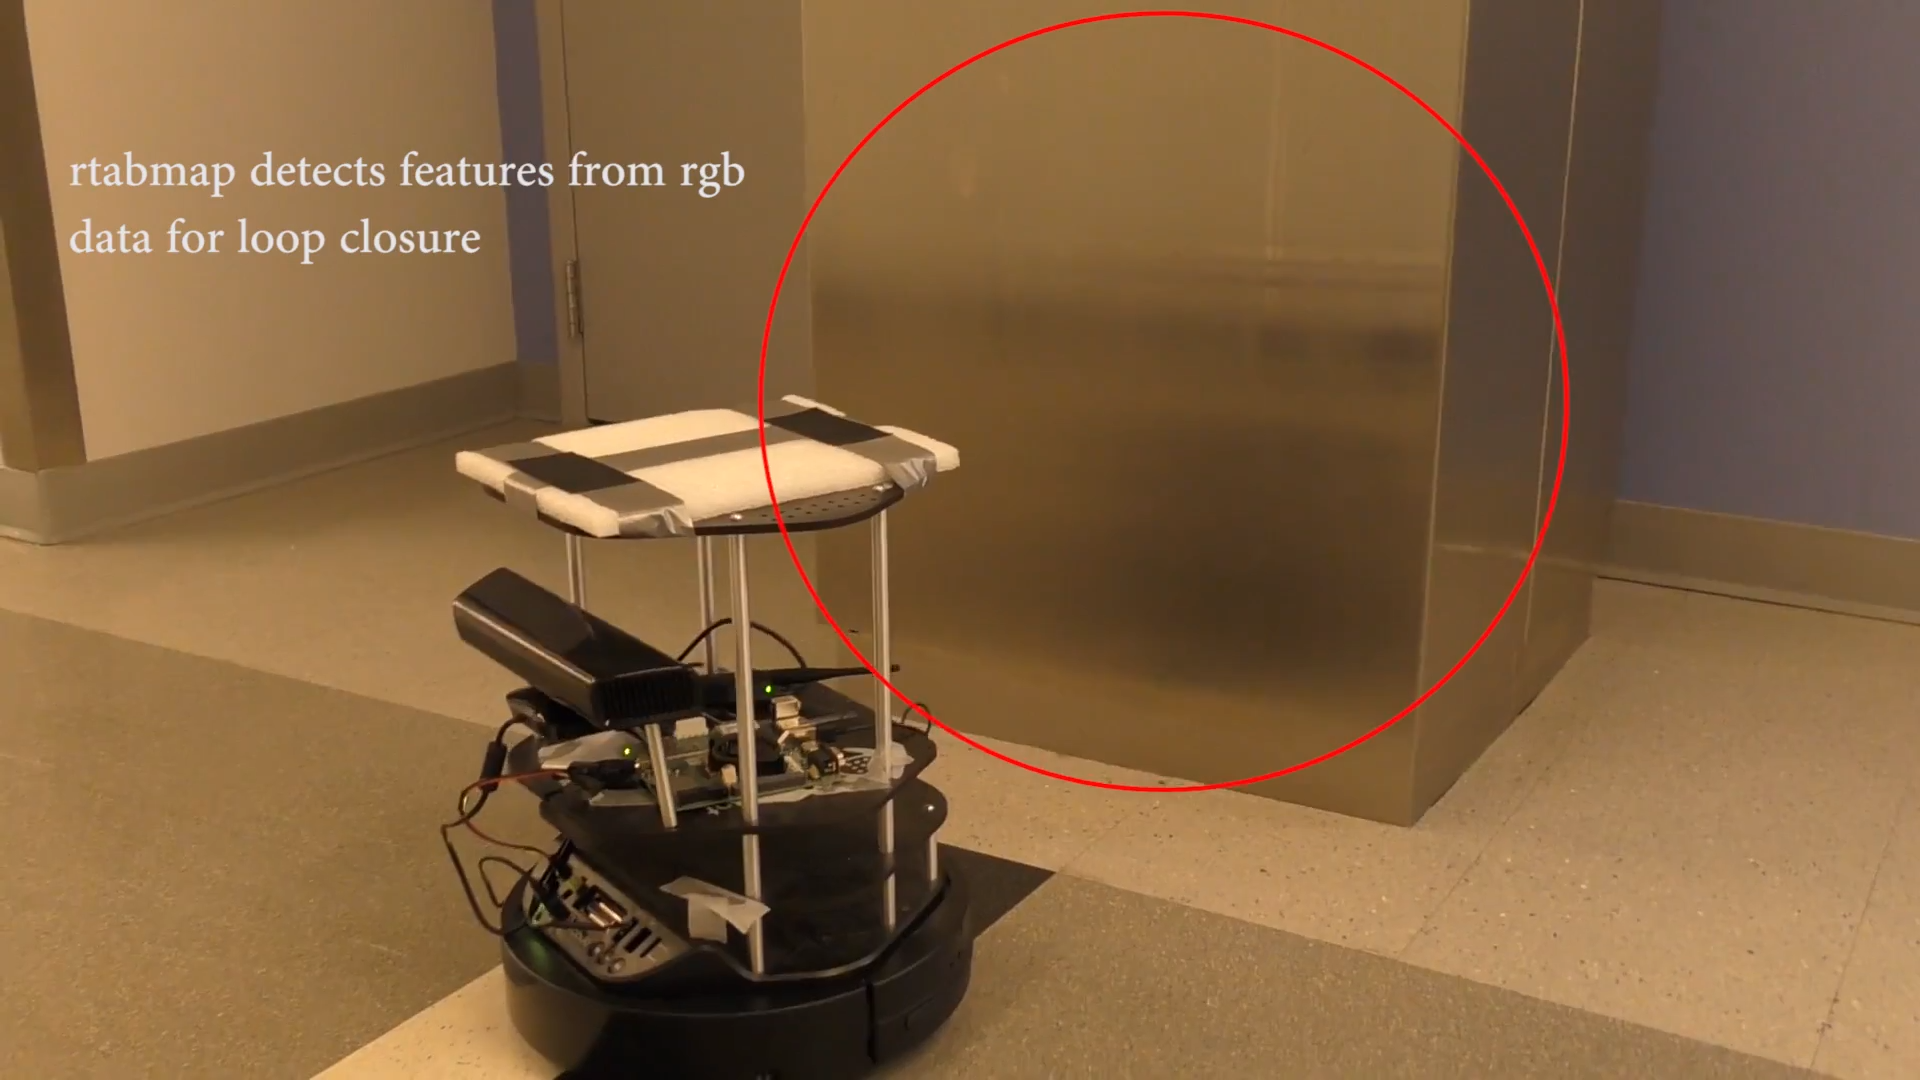
\includegraphics[width=\textwidth, height=0.7\textwidth]{images/loop1.png}
		\label{subfig:a}
		\caption{RTAB-Map processing RGB features from the sensor data.}
		\vspace{2em}
	\end{subfigure}
	\begin{subfigure}[b]{0.497\textwidth}
		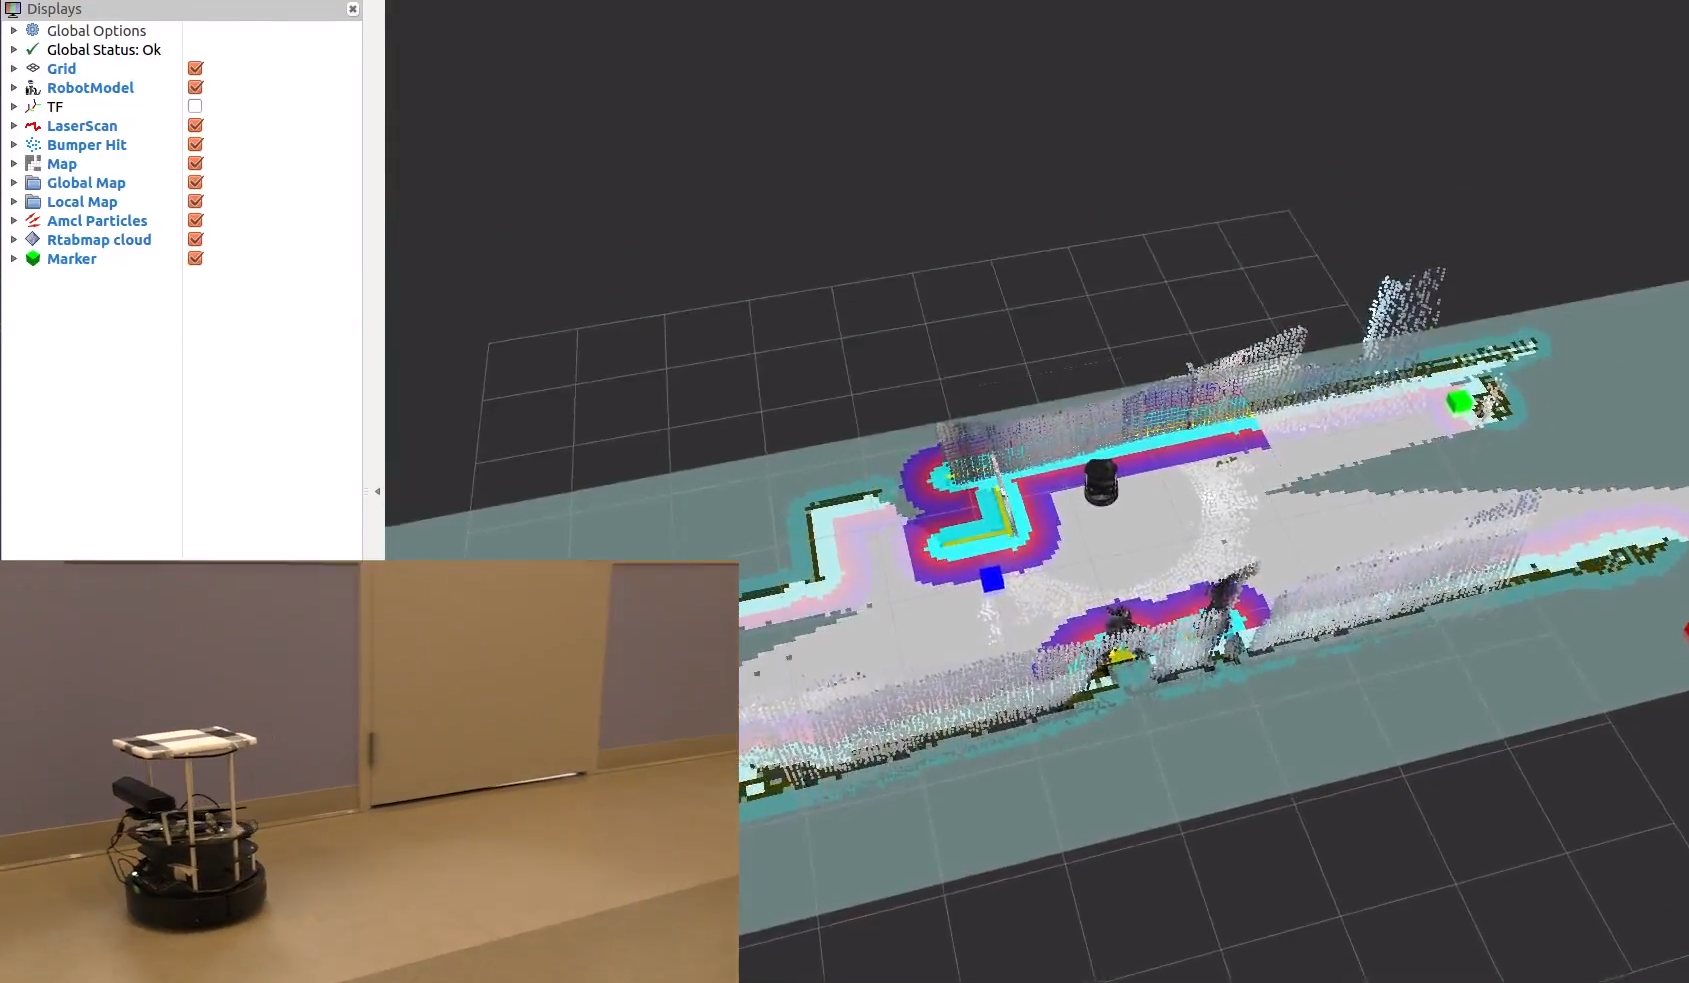
\includegraphics[width=\textwidth, height=0.7\textwidth]{images/loop2.png}
		\label{subfig:b}
		\caption{Turtlebot moving to the next best frontier point indicated as green cube.}
		\vspace{2em}
	\end{subfigure}
% 	\hfill
	\begin{subfigure}[b]{0.497\textwidth}
		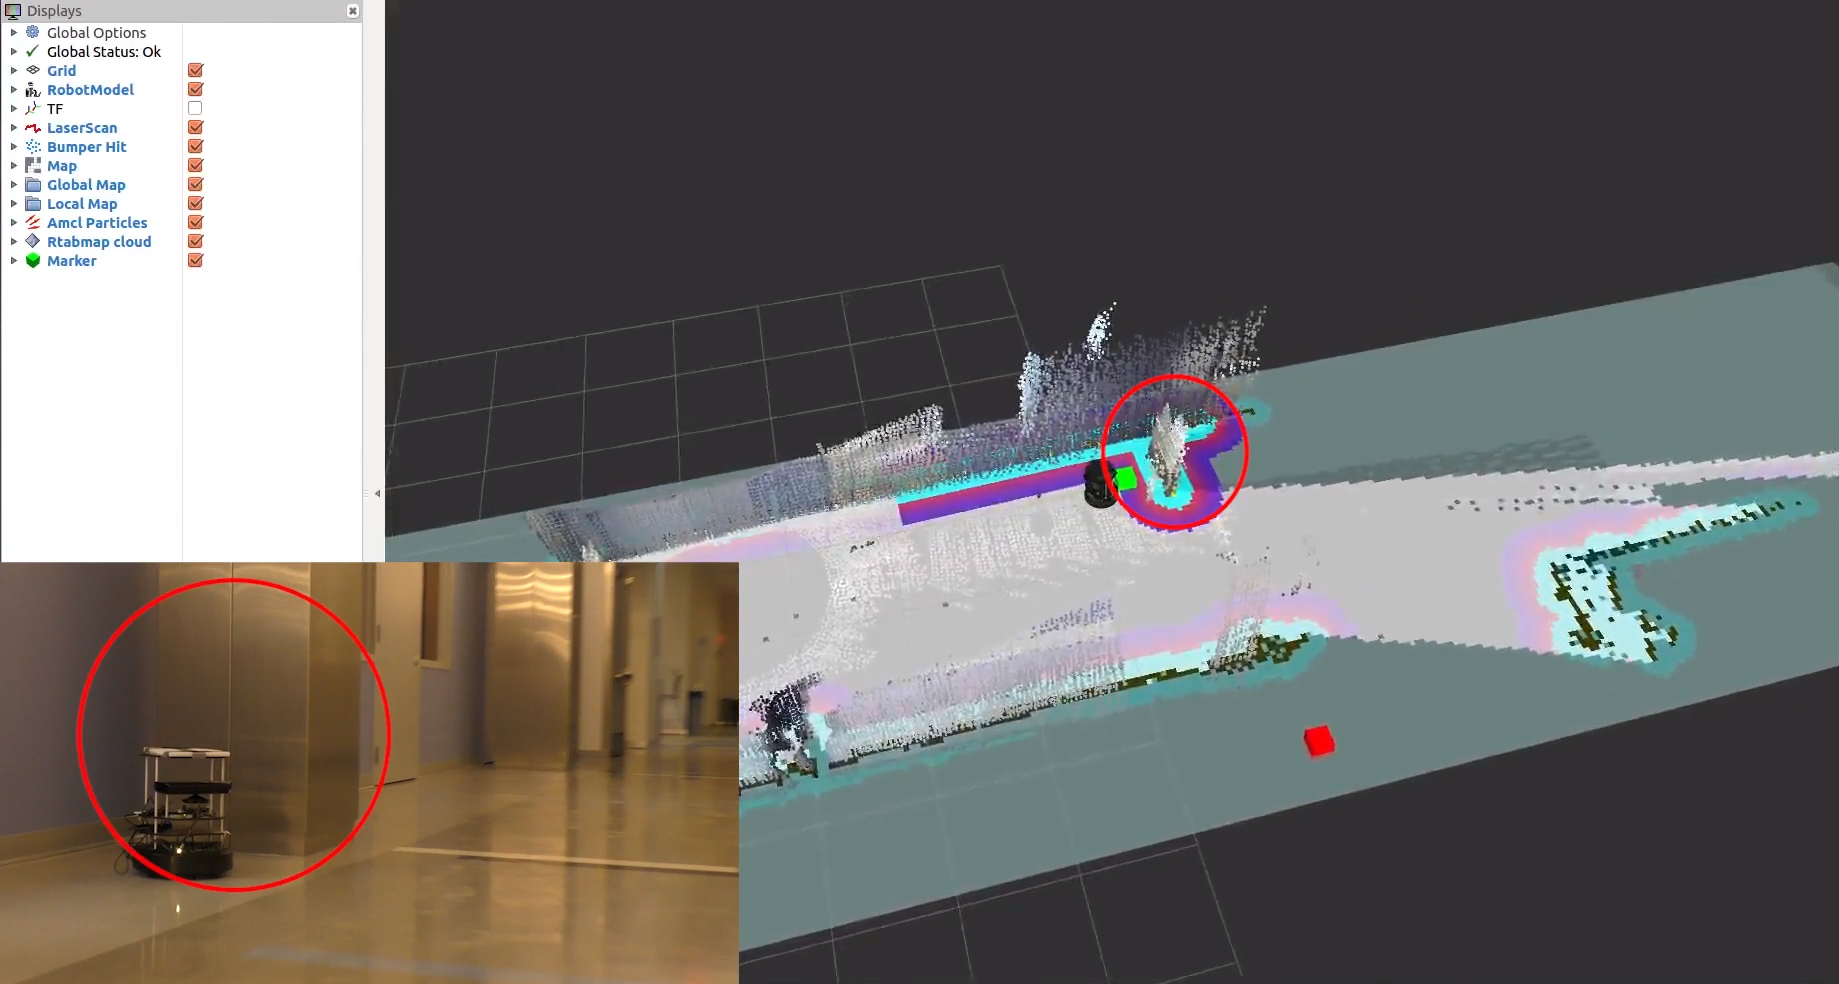
\includegraphics[width=\textwidth, height=0.7\textwidth]{images/loop3.png}
		\label{subfig:c}
		\caption{RTAB-Map detects similarities in features with that of in the previous scene.}
	\end{subfigure}
    % \vfill
	\begin{subfigure}[b]{0.497\textwidth}
		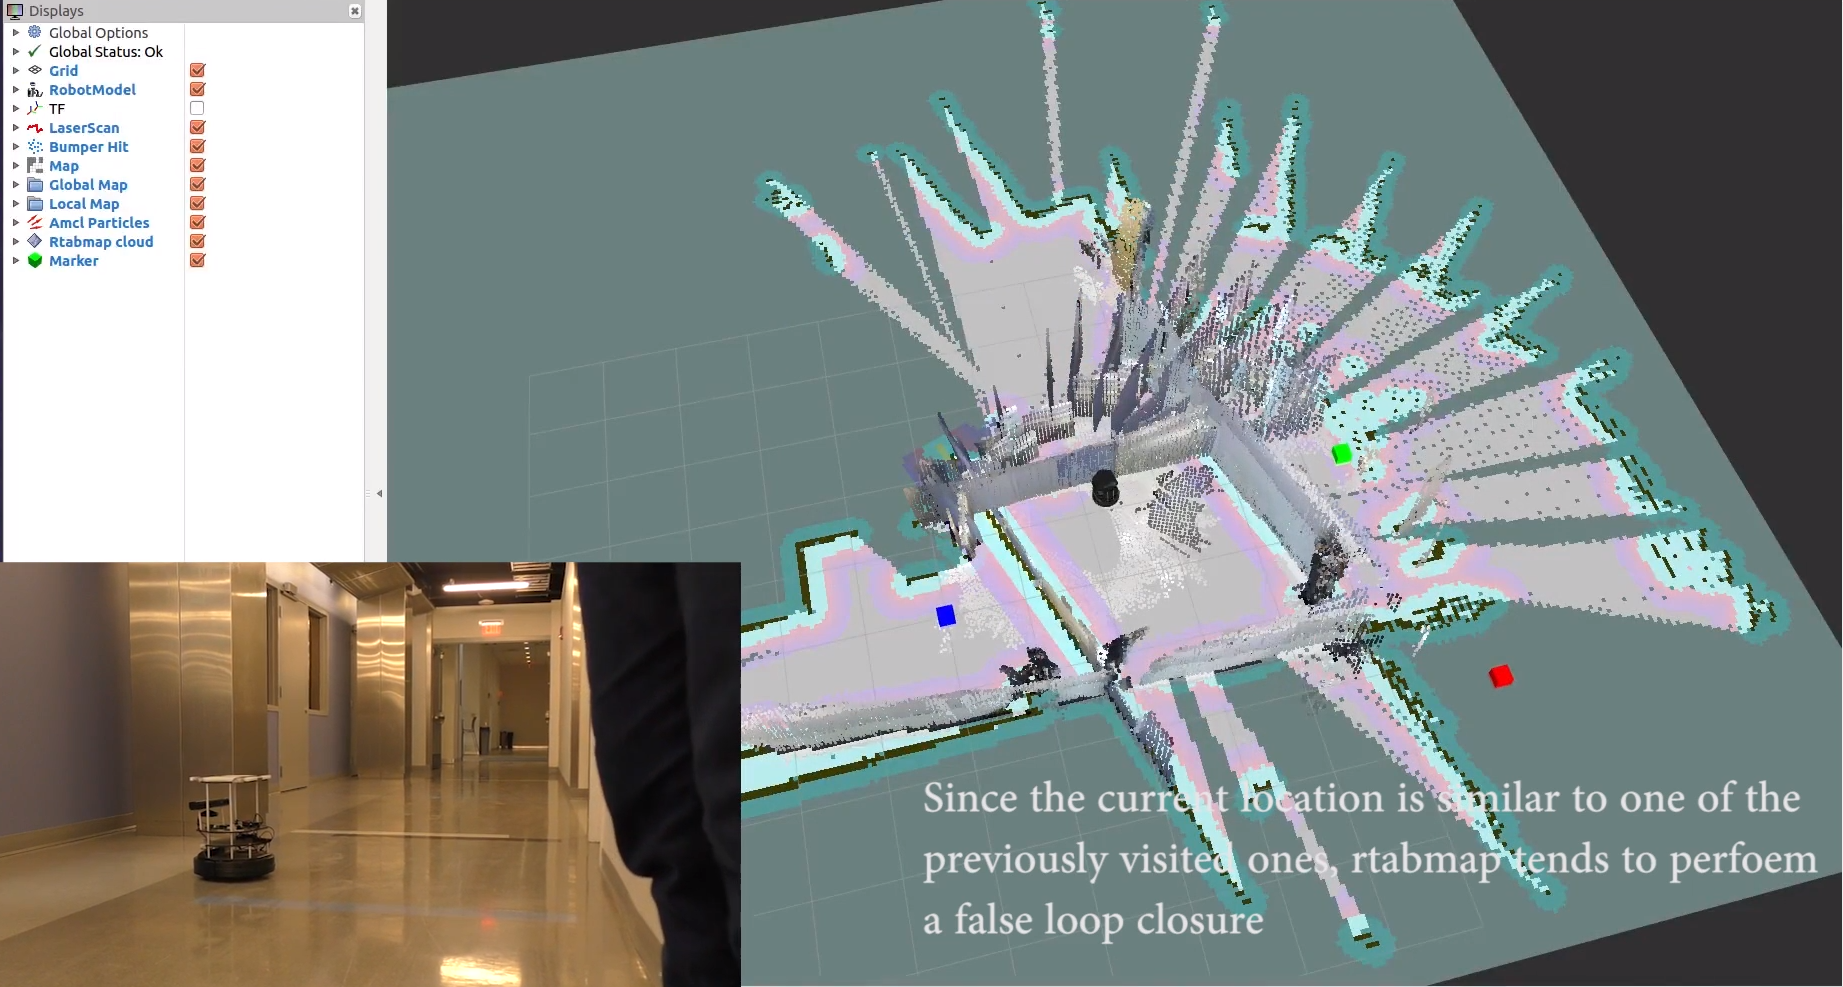
\includegraphics[width=\textwidth, height=0.7\textwidth]{images/loop4.png}
		\label{subfig:d}
		\caption{Performs a false loop closure. Turtlebot's pose is changed and map is erroneously updated.}
	\end{subfigure}
\caption{Demonstrates a false loop closure using RTAB-Map}
\end{figure*}

\clearpage
\textbf{Solution}:
Visual SLAM algorithms such as RTAB-Map use memory schemes to eliminate false loop closures\cite{22} which work well in real time but does have edge cases which can fail the algorithm. For instance, if the robot has to map a very long corridor, a possibility exist that the feature has been moved to long term memory making the robot incapable to close the loop when the start point is revisited.

\subsection{Sensor shortcomings}
Kinect’s impact has extended far beyond the gaming industry\cite{24}. With its wide availability and low cost, many researchers and practitioners in computer science, electronic engineering, and robotics are leveraging the sensing technology to develop creative new ways to interact with machines and to perform other tasks, such as mapping an unknown environment. Technical specifications of this device has been listed in chapter 3. But it comes with its own shortcomings as well. Sensor like Kinect is incapable of detecting thin obstacles such as chair legs etc especially when the object falls below 0.8m range. Fig 4.18 shows a failed test run where the Turtlebot bumped into a chair and handicapped itself.

\begin{figure*}[!h]
\centering
	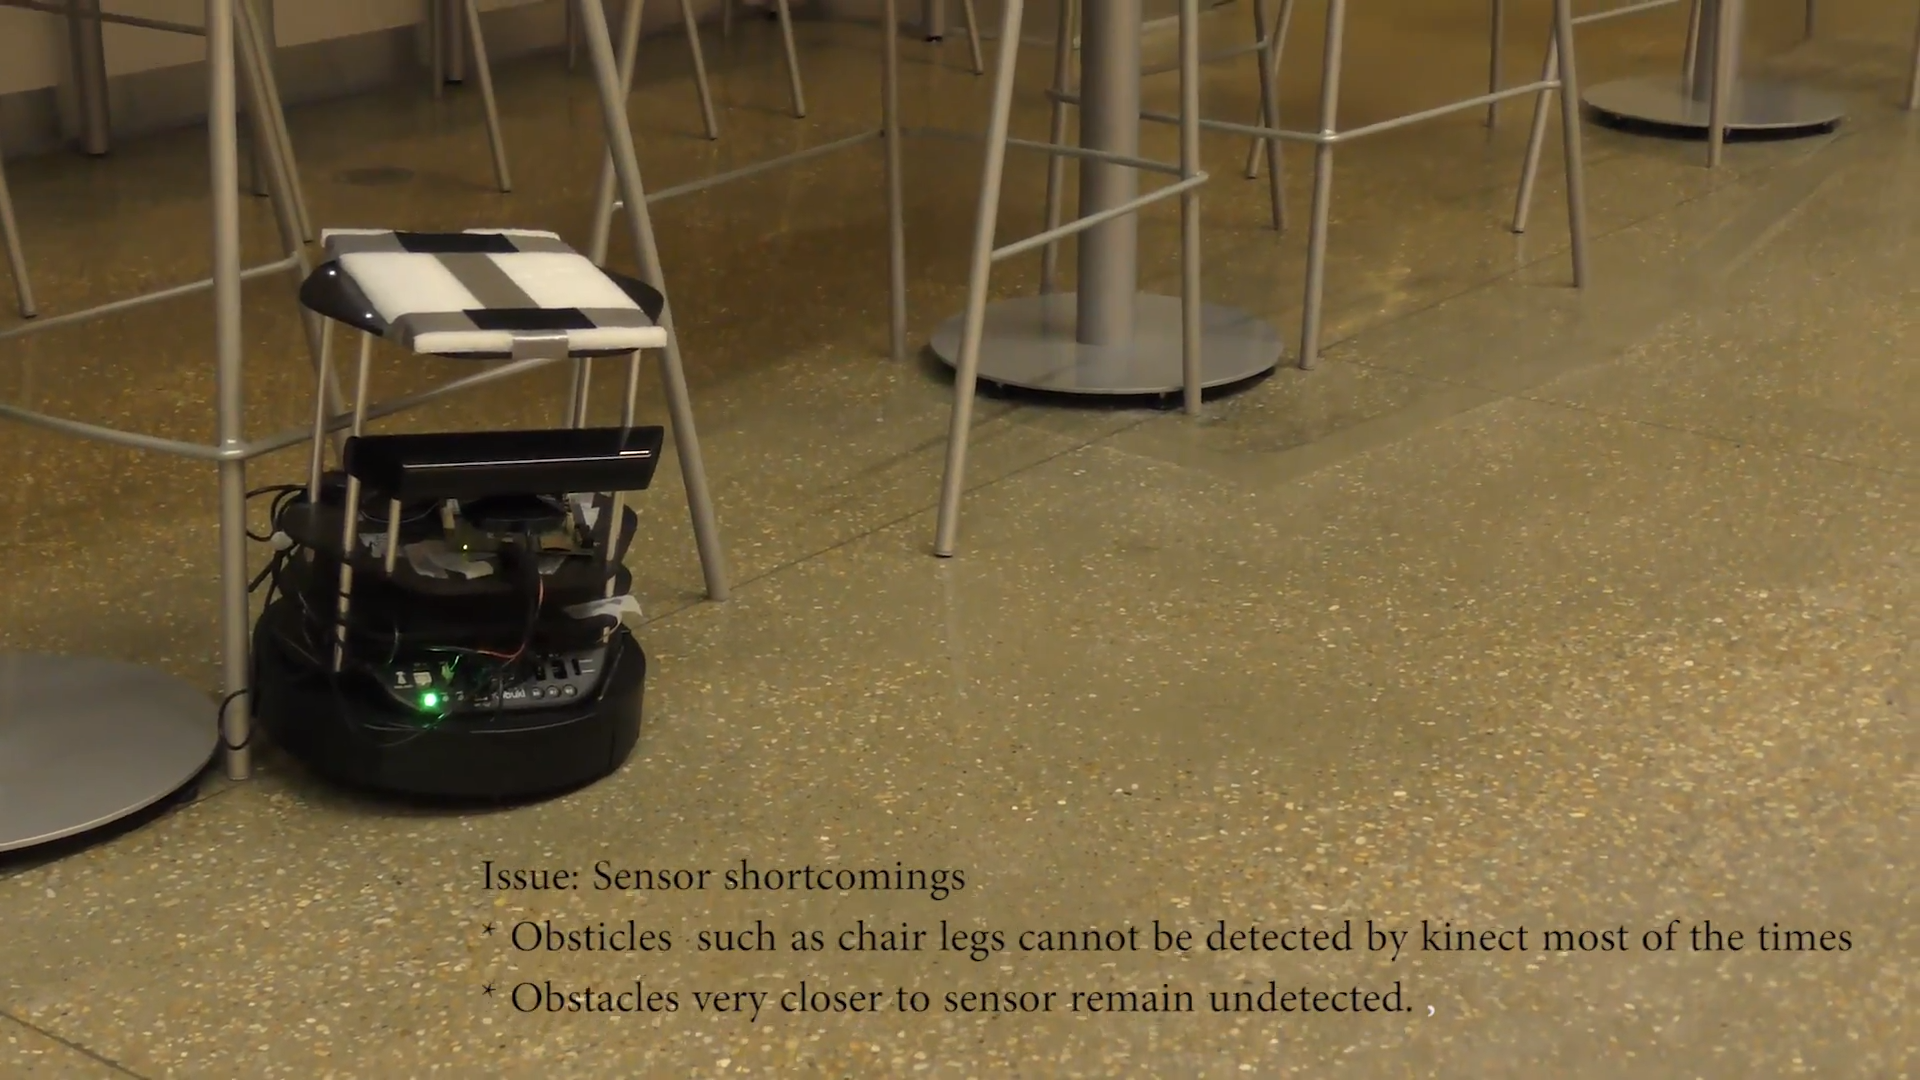
\includegraphics[width=0.75\textwidth]{images/chairleg.png}
\caption{Image shows a Turtlebot getting stuck after bumping into a chair}
\end{figure*}

\subsection{Obstacles}
Due to occupancy grid resolution from RTAB-Map being extremely high, i.e 0.05m, the obstacles detected rise sharp from the empty. The potential problem occurs when the next best position selected is close to the obstacle. In such case, the robot often hits the obstacles in order to move to an unreachable position relative to its foot print. 

\textbf{Solution}: Inflating the obstacles and filtering the potential unreachable frontiers can eliminate the problem. Fig 4.19(A) shows the obstacles identified from the occupancy grid. Gaussian smoothing has been applied to the obstacles and the original obstacle depths are superimposed onto the smoothed obstacles as shown in Fig 4.19(B). Frontiers lying in the gaussian zone are eliminated preventing the risk of robot hitting the obstacle or getting stuck near it.

\begin{figure*}
    \begin{subfigure}[b]{0.498\textwidth}
		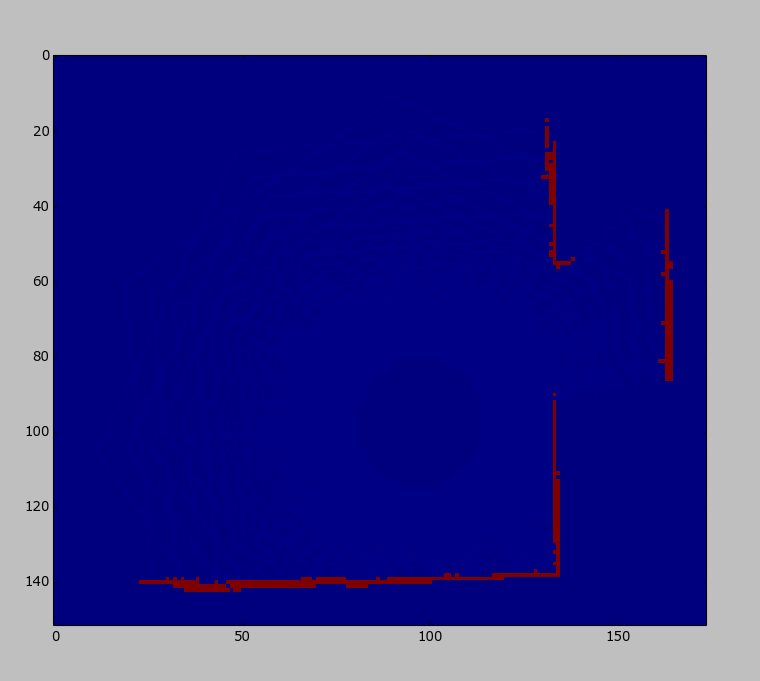
\includegraphics[width=\textwidth, height=\textwidth]{images/inflation.png}
		\label{subfig:a}
		\caption{}
	\end{subfigure}
	\begin{subfigure}[b]{0.498\textwidth}
		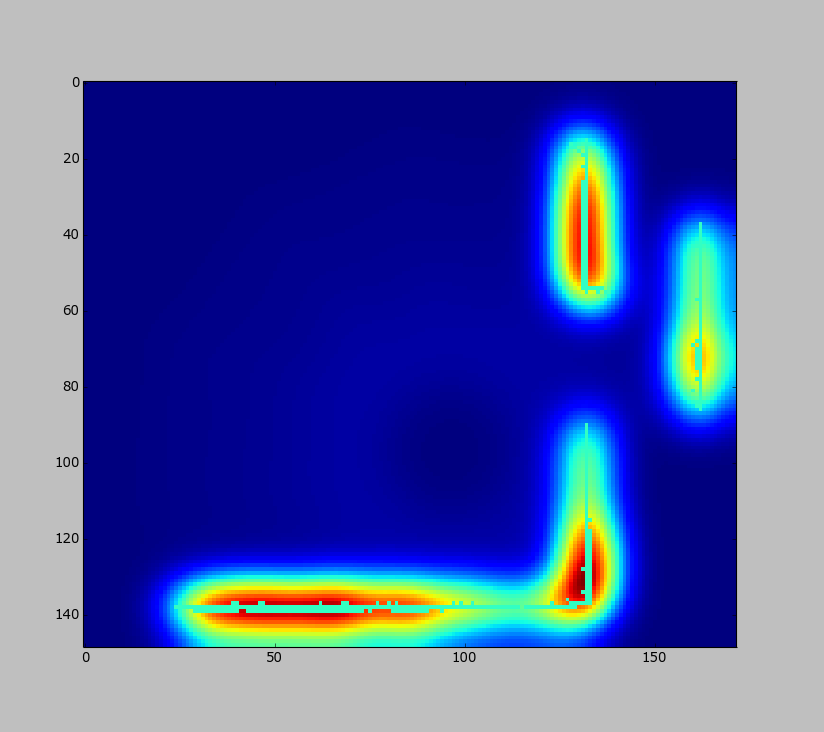
\includegraphics[width=\textwidth, height=\textwidth]{images/inflated_obs.png}
		\label{subfig:b}
		\caption{}
	\end{subfigure}
\caption{Inflation of obstacles}
\end{figure*}




























